\documentclass[
  aspectratio=1610,
]{beamer}

%\includeonlyframes{current,other}

\usepackage[american]{babel}
\usepackage[utf8]{inputenc}
\usepackage[T1]{fontenc}

% needs https://tex.stackexchange.com/questions/423848/xelatex-xy-and-dejavu-otf#423854
%\usepackage{dejavu-otf} % default Makie font: DejaVu Sans
%\usefonttheme{professionalfonts}

\title{A Low-Rank Parareal Solver for\\ Differential Riccati Equations\\ Written in Julia}
\author{Jonas Schulze}
\institute{Faculty of Mathematics\\ Otto-von-Guericke-Universität Magdeburg}
\date{May 10, 2022}
\subject{subject}

% beamer appearance
\setbeamercolor{block body}{bg=mpi} % for debugging
\setbeamercovered{transparent}
\beamertemplatenavigationsymbolsempty

\newcommand\maketocframe[1][]{%
  \begin{frame}{Outline}
    \tableofcontents[#1]
  \end{frame}
}

\AtBeginSection{%
  \maketocframe[currentsection,currentsubsection]
}

\usepackage[
  style=authoryear,
]{biblatex}
\addbibresource{stuff.bib}

\usepackage{mathtools}
\usepackage{xparse,xspace}
\usepackage{booktabs}
\usepackage{csquotes}
\usepackage[shortcuts]{glossaries}
\usepackage[binary-units]{siunitx}
\usepackage{listings}

\lstset{
  basicstyle=\small\ttfamily\color{black!15}, % should match transparency of covered
  columns=flexible,
}

\usepackage{tikz}
\usetikzlibrary{positioning}
\usetikzlibrary{graphs,arrows.meta}
\tikzset{>=Stealth}

\sisetup{
  round-mode = places,
  round-precision = 2,
}

\newcommand{\N}{\mathbb{N}} % Natural numbers
\newcommand{\Z}{\mathbb{Z}} % Whole numbers
\newcommand{\Q}{\mathbb{Q}} % Rational numbers
\newcommand{\R}{\mathbb{R}} % Real numbers
\newcommand{\C}{\mathbb{C}} % Complex numbers
\newcommand{\F}{\mathbb{F}} % Arbitrary Field
\newcommand{\K}{\mathbb{K}} % Arbitrary Field

\newcommand{\Cneg}{\C_-} % Negative Half Plane

\newcommand{\im}{i} % imaginary unit

\newcommand{\onehalf}{\tfrac{1}{2}}

% matrices
\newcommand\Cnn{\C^{n\times n}}
\newcommand\Rnn{\R^{n\times n}}
\newcommand\Rnr{\R^{n\times r}}
\newcommand\Rnk{\R^{n\times k}}
\newcommand\Rkk{\R^{k\times k}}
\newcommand\nnz{\operatorname{nnz}}
\renewcommand\vec{\operatorname{vec}}
\DeclareMathOperator{\colspan}{span}
\DeclareMathOperator{\orth}{orth}
\DeclareMathOperator{\rank}{rank}
\DeclareMathOperator{\diag}{diag}
\newcommand\MP{\dagger} % Moore Penrose pseudo-inverse

% transpose and conjugate/Hermitian transpose:
\newcommand\conj[1]{\overline{\optional{#1}}}
\newcommand\T{T}
\newcommand\HT{H}

% Rosenbrock
\newcommand\Ham{\ensuremath{H}}
\newcommand\Ricc{\operatorname{\mathcal R}}
\newcommand\Jac{\operatorname{\mathcal J}}

 % ADI
\newcommand\Aip{\mathop{H_k^+}}
\newcommand\Aim{\mathop{H_k^-}}
\newcommand\Aipm{\mathop{H_k^\pm}}
\newcommand\Aiip{\mathop{V_k^+}}
\newcommand\Aiim{\mathop{V_k^-}}
\newcommand\Aiipm{\mathop{V_k^\pm}}
\newcommand\Cayley{\mathop{\mathcal{C}}}
\newcommand\Aipinv{\mathop{(\Aip)^{-1}}}
\newcommand\Aiipinv{\mathop{(\Aiip)^{-1}}}
\newcommand\Lyap{\operatorname{\mathcal L}}

% usage: \{2x\given x\in\N}
\newcommand{\given}{\mid}

% usage: \Set[\big]{2x \given x\in\N}
\newcommand\SetSymbol[1][]{%
  \nonscript\:#1\vert
  \allowbreak
  \nonscript\:
  \mathopen{}}
\DeclarePairedDelimiterX{\Set}[1]{\lbrace}{\rbrace}{%
  \renewcommand\given{\SetSymbol[\delimsize]}% this effect is local only
  #1%
}

% personal taste:
\let\epsilon\varepsilon
%\renewcommand{\to}{\longrightarrow}
%\renewcommand{\mapsto}{\longmapsto}
%\renewcommand{\gets}{\longleftarrow}
\renewcommand{\Re}{\operatorname{Re}} % real part of a complex number
\renewcommand{\Im}{\operatorname{Im}} % imaginary part

% some more delimiters:
\NewDocumentCommand{\optional}{m}{\ifblank{#1}{\,\cdot\,}{#1}}
\DeclarePairedDelimiterX{\abs}[1]{\lvert}{\rvert}{\optional{#1}}
\DeclarePairedDelimiterX{\norm}[1]{\lVert}{\rVert}{\optional{#1}}
\DeclarePairedDelimiterX{\scalar}[2]{\langle}{\rangle}{\optional{#1},\optional{#2}}
\newcommand{\card}{\abs}

% integration:
\NewDocumentCommand{\intd}{m}{\,\textup{d}#1}
\newcommand\dt{\intd{t}}

% differentiation:
\NewDocumentCommand{\pdiff}{mm}{\frac{\partial #2}{\partial #1}}
\NewDocumentCommand{\diff}{mm}{\frac{\mathrm{d} #2}{\mathrm{d} #1}}

\newcommand\julia\texttt
\newcommand\code\texttt

\newcommand\LDLt{LDL\textsuperscript{T}}

\counterwithout*{footnote}{chapter}
\setcounter{topnumber}{1} % max number of floats at top of page
\renewcommand{\bottomfraction}{0.5}
\renewcommand{\listtheoremname}{List of Theorems and Examples}

\newcommand\LandauO{\operatorname{\mathcal O}}

% runtime estimates
\newcommand\hattpar{\hat t_\text{par}} % estimate
\newcommand\hattseq{\hat t_\text{seq}} % estimate
\newcommand\tpar{t_\text{par}}
\newcommand\tseq{t_\text{seq}}
\newcommand\twarmup{t_\text{warm-up}}
\newcommand\trampup{t_\text{ramp-up}}
\newcommand\JIT{\operatorname{compile}}

% error estimates
\newcommand\umach{\mathrm u_\text{mach}} % machine precision

% https://tex.stackexchange.com/questions/22561/what-is-the-proper-use-of-i-e-backslash-at?noredirect=1&lq=1
\makeatletter % no idea why this is needed. \@ifnextchar doesn't work without it.
\newcommand\cf{cf.\@\xspace} % confer
\newcommand\eg{e.g.\@\xspace} % exempli gratia
\newcommand\etc{etc\@ifnextchar.{}{.\@\xspace}} % et cetera
\newcommand\ie{i.e.\@\xspace} % id est
\newcommand\wrt{w.r.t.\@\xspace} % with respect to
\makeatother

\definecolor{mathcore} {RGB}{102,  99, 100}
\definecolor{ovgu math}{RGB}{209,  63,  88}
\definecolor{mpi}      {RGB}{ 61, 167, 197}
\def\cola{ovgu math}
\def\colb{mathcore}
\def\colc{mpi}

\tikzset{
  mat/.style={
    rectangle,
    minimum size=1ex,
    inner sep=0mm,
  },
  bigmat/.style={mat,minimum size=#1},
  bigmat/.default=1cm,
  tallmat/.style={mat,minimum height=#1},
  tallmat/.default=1cm,
  widemat/.style={mat,minimum width=#1},
  widemat/.default=1cm,
  smallmat/.style={mat},
}

\newcommand\mat[2]{%
  \tikz[baseline=(M.base)] \node [mat, #1, fill=ovgu math] (M) {$#2$};
}
\newcommand\bigmat[1]{\mat{minimum size=2cm}{#1}}
\newcommand\tallmat[2][6mm]{\mat{minimum size=#1, minimum height=2cm}{#2}}
\newcommand\widemat[2][6mm]{\mat{minimum size=#1, minimum width=2cm}{#2}}
\newcommand\smallmat[2][6mm]{\mat{minimum size=#1}{#2}}

\newcommand\tallcmat[1]{\tikz[baseline=-0.5ex]\node[tallmat,fill=#1] {};}
\newcommand\smallcmat[1]{\tikz\node[smallmat,fill=#1] {};}
\newcommand\widecmat[1]{\tikz\node[widemat,fill=#1] {};}
\newcommand\colorldlt[1]{%
  \mathop{\tallcmat{#1}}
  \mathop{\smallcmat{#1}}
  \mathop{\widecmat{#1}}
}

\newcommand\colorspacing{%
  \arraycolsep=3pt
  \def\arraystretch{0.75}
}


\renewcommand\mathrm\mathsf % fix \umach
\newcommand\emptyblock[1]{%
  \begin{beamercolorbox}{block title}
    \usebeamerfont{block title}%
    #1
  \end{beamercolorbox}
}

%TODO: what if the frame needs multiple slides?
\newcommand\bigpicture[1]{%
  \onslide
  \setcounter{beamerpauses}{1}
  \begin{block}{Big Picture}
    \begin{itemize}
      \item
        Differential \Riccati Equation (DRE)
      \ifnum#1<2 \pause\fi
      \item
        Solution in LRSIF
      \ifnum#1<3 \pause\fi
      \item
        Rosenbrock method\\ to solve DRE
      \ifnum#1<4 \pause\fi
      \item
        Rosenbrock stages are ALEs
      \ifnum#1<5 \pause\fi
      \item
        ADI method\\ to solve ALE
      \ifnum#1<6 \pause\fi
      \item
        Parareal method\\ for speed-up
    \end{itemize}
  \end{block}
}

\newcommand\tallcmat[1]{\tikz[baseline=-0.5ex]\node[tallmat,fill=#1] {};}
\newcommand\smallcmat[1]{\tikz\node[smallmat,fill=#1] {};}
\newcommand\widecmat[1]{\tikz\node[widemat,fill=#1] {};}
\newcommand\colorldlt[1]{%
  \mathop{\tallcmat{#1}}
  \mathop{\smallcmat{#1}}
  \mathop{\widecmat{#1}}
}

\newcommand\colorspacing{%
  \arraycolsep=3pt
  \def\arraystretch{0.75}
}

\begin{document}

\frame[plain]{\titlepage}
\maketocframe

\everymath{\displaystyle}

\section{Motivation}

\begin{frame}{Motivation}
  \begin{columns}[t,onlytextwidth]
  \column{0.5\linewidth}
  \begin{block}{\strut Optimal Control Problem}
    Consider the \acf{LQR} problem
    \begin{equation*}
      \begin{array}{cl}
        \min_u & \int_{t_0}^{t_f} y^\T y + u^\T u \dt + \tfrac{1}{100} y(t_f)^\T y(t_f) \medskip\\
        \text{s.t.} & \begin{aligned}[t]
          E \dot x &= Ax + Bu \\
          y &= Cx
        \end{aligned}
      \end{array}
    \end{equation*}
    using
    \begin{itemize}
      \item
        state $x(t)\in\R^n$
      \item
        control $u(t)\in\R^m$, $m\ll n$
      \item
        output $y(t)\in\R^q$, $q\ll n$
      \item
        constant system matrices $E,A,B,C$.
    \end{itemize}
  \end{block}
  \pause
  \column{0.47\linewidth}
  \begin{block}{\strut Feedback Law \parencite[e.g.][]{Locatelli2011}}
    The optimal control is given by
    \begin{equation*}
      u(t) = -
        B^\T X(t_f+t_0-t) E
      x(t)
    \end{equation*}
    where $X(t)\in\R^{n\times n}$ solves the \acf{DRE}
    \begin{equation*}
      \left\{
        \begin{lgathered}
          E\dot X E = \begin{multlined}[t]
            C^\T C + A^\T X E + E^\T X A \\ - E^\T X BB^\T X E
          \end{multlined} \\
          E^\T X(t_0) E = \tfrac{1}{100} C^\T C
          .
        \end{lgathered}
      \right.
    \end{equation*}
  \end{block}
  \end{columns}
\end{frame}

\begin{frame}{Oberwolfach Rail}
\begin{columns}[onlytextwidth]
\column{0.6\textwidth}
  \begin{itemize}
    \item
      \cite{Benner2005}
    \item
      Linearized 2D heat equation:
      \begin{align*}
        c \rho\, \partial_t x &= \lambda\,\Delta x, && x\in\Omega\\
        \lambda\, \partial_n x &= q_k (u_k - x), && x \in\Gamma_k, k=1,\ldots,7\\
        \partial_n x &= 0, && x\in\Gamma_0
      \end{align*}
    \item
      FEM discretizations / mesh refinements with
      $n\in\Set{371,1357,5177,\num{20209},\ldots}$ states,\\
      $m=7$ inputs,
      $q=6$ outputs
    \item
      Time horizon $t\in[\SI{0}{\second}, \SI{45}{\second}]$
    \item
      Resulting $(E, A, B, C)$ system:
      $E \succ 0$ and $A \prec 0$\\
      $\leadsto$ uniquely solvable
  \end{itemize}
\column{0.37\textwidth}
  \includegraphics[width=\textwidth]{figures/Steelprofile1.jpg}
\end{columns}
\end{frame}

\begin{frame}<1>{Motivation}
\begin{bigpicturecols}
  \begin{itemize}
    \item
      Large-scale problems: a single (dense) $X(t)\in\Rnn$\\
      takes \SI{200}{\tera\byte} for
      $n=\num{5000000}$
    \item
      Solution $X$ is symmetric and dense, but has low rank

      \parencite[e.g.][]{Penzl2000}
    \item[$\leadsto$]
      Approximation via \rlap{\acl{LRSIF}:}
      \begin{equation*}
        \bigmat{X} \approx \mathop{\tallmat{L}} \mathop{\smallmat{D}} \mathop{\widemat{L^{\smash{\T}}}}
      \end{equation*}
    \item
      DRE is highly stiff, \ie\\
      high accuracy requires small time steps or high orders
    \item[$\leadsto$]
      Parareal method for speed-up
  \end{itemize}
\column{\bigpicturewidth}
\bigpicture{1}
\end{bigpicturecols}
\end{frame}


\section{Next}

\subsection{Low-Rank Symmetric Indefinite Factorization}

\begin{frame}<1>{Low-Rank Symmetric Indefinite Factorization (LRSIF)}
\begin{bigpicturecols}
  \begin{itemize}
    \item
      \cite{Benner2009}
    \item
      Arithmetic:
      \begin{equation*}
        \colorspacing
        \colorldlt{\cola} \pm \colorldlt{\colc}
        :=
        \Bigg[
        \begin{matrix}
          \tallcmat{\cola} &
          \tallcmat{\colc}
        \end{matrix}
        \Bigg]
        \begin{bmatrix}
          \smallcmat{\cola} \\
          & \pm \smallcmat{\colc}
        \end{bmatrix}
        % flag of the Netherlands:
        \begin{bmatrix}
          \widecmat{\cola} \\
          \widecmat{\colc}
        \end{bmatrix}
      \end{equation*}
    \item
      Problem: growing storage requirements, \eg
      \begin{equation*}
        \colorspacing
        \colorldlt{\cola} + \colorldlt{\cola}
        :=
        \Bigg[
        \begin{matrix}
          \tallcmat{\cola} &
          \tallcmat{\cola}
        \end{matrix}
        \Bigg]
        \begin{bmatrix}
          \smallcmat{\cola} \\
          & \smallcmat{\cola}
        \end{bmatrix}
        % flag of Austria:
        \begin{bmatrix}
          \widecmat{\cola} \\
          \widecmat{\cola}
        \end{bmatrix}
        %\not\equiv
        %\mathop{\tallcmat{\cola}}
        %\mathop{(\smallcmat{\cola} + \smallcmat{\cola})}
        %\mathop{\widecmat{\cola}}
      \end{equation*}
      $\leadsto$ compression necessary
      (how: \cite{Lang2017})
    \item
      Note: \enquote{low-rank} versions of a matrix or algorithm refer to \enquote{LRSIF}
  \end{itemize}
\column{\bigpicturewidth}
\bigpicture{2}
\end{bigpicturecols}
\end{frame}

\subsection{Rosenbrock Method}

\begin{frame}<1>{Rosenbrock Method}
\begin{columns}
\column{0.7\textwidth}
  \begin{block}{General Formulation}
    For the initial value problem (IVP) $\dot x = f(x)$ the method reads
    \begin{equation*}
    \left\{
    \begin{aligned}
      x_{n+1} &:= x_n + \tau \sum_{j=1}^s b_j k_j
      \\
      k_i &:= \begin{multlined}[t]
      f\left( x_n + \tau \sum_{j=1}^{i-1} \alpha_{ij} k_j \right) + \tau \Jac \sum_{j=1}^i \gamma_{ij} k_j
      \\
      \text{for } i = 1, \ldots, s
      ,
      \end{multlined}
    \end{aligned}
    \right.
    \end{equation*}
    where $\Jac := f'(x_n)$ denotes the Jacobian.
  \end{block}
\column{0.3\textwidth}
\bigpicture{3}
\end{columns}
\end{frame}

\begin{frame}<1>{Rosenbrock Method}
\begin{columns}
\column{0.7\textwidth}
  \begin{block}{1st Order Scheme (Linearly Implicit Euler Scheme)}
    For the IVP $\dot x = f(x)$ the method reads
    \begin{equation*}
    \left\{
    \begin{aligned}
      x_{n+1} &= x_n + \tau k_1 \\
      (I - \gamma\tau \Jac) k_1 &= f(x_n)
      .
    \end{aligned}
    \right.
    \end{equation*}
  \end{block}
  \begin{block}{2nd Order Scheme \parencite{Verwer1999}}
    %\vspace*{-\baselineskip}
    %For the IVP $\dot x = f(x)$ the method reads
    \begin{equation*}
    \left\{
    \begin{aligned}
      x_{n+1} &= x_n + \tfrac{3}{2} \tau k_1 + \tfrac{1}{2} \tau k_2 \\
      (I - \gamma\tau \Jac) k_1 &= f(x_n) \\
      (I - \gamma\tau \Jac) k_2 &= f(x_n + \tau k_1) - 2k_1
    \end{aligned}
    \right.
    \end{equation*}
  \end{block}
\column{0.3\textwidth}
\bigpicture{3}
\end{columns}
\end{frame}

\begin{frame}<-4>{Rosenbrock Method}
\begin{columns}
\column{0.7\textwidth}
\begin{itemize}
\item
  Consider the DRE $E^\T \dot X E = \Ricc(X)$.
  \newcommand\U{\alert{\makebox[\widthof{$X_n$}]{$U$}}}
  \begin{align*}
    \Ricc(X_n) &= C^\T C + A^\T X_n E + E^\T X_n A - E^\T X_n BB^\T X_n E
    \\
    \pause
    \Jac(\alert{U}) &= \makebox[\widthof{$C^\T C$}]{$0$}
      + A^\T \U E + E^\T \U A
      \begin{lgathered}[t]
        {} - E^\T \U BB^\T X_n E \\
        {} - E^\T X_n BB^\T \U E
      \end{lgathered} \\
    \pause
    &= (A - BB^\T X_n E)^\T \alert U E + E^\T \alert U (A - BB^\T X_n E)
  \end{align*}
\item
  The Jacobian is a Lyapunov operator!
\pause
\item %TODO: when \leadsto, when \implies?
  $I - \gamma\tau\Jac$ is a Lyapunov operator,
  \ie all Rosenbrock stages are Algebraic Lyapunov Equations (ALEs).
\end{itemize}
\column{0.3\textwidth}
\bigpicture[3]{3}
\end{columns}
\end{frame}

\begin{frame}<1>{1st Order Rosenbrock Scheme}
\begin{columns}
\column{0.7\textwidth}
  \begin{itemize}
    \item
      Linearly implicit Euler scheme
    \item
      \cite{Mena2007}: Formulation for DRE $E^\T \dot X E = \Ricc(X)$
    \item
      \cite{Lang2017}: Formulation for LRSIF $X(t) = LDL^\T$
    \item
      1 ALE per step:
      \begin{equation*}
        \tilde A_n^\T X_{n+1} E + E^\T X_{n+1} \tilde A_n = - GSG^\T
      \end{equation*}
      where
      \begin{align*}
        \tilde A_n &= \gamma\tau(A-BB^\T X_n E) - \tfrac{1}{2} E
        \\
        G &= \begin{bmatrix}
          C^\T & E^\T L
        \end{bmatrix}
        \\
        S &= \begin{bmatrix}
          I & . \\
          . & DL^\T BB^\T LD + \tfrac{1}{\tau} D
        \end{bmatrix}
      \end{align*}
  \end{itemize}
  \vfill
\column{0.3\textwidth}
\bigpicture{4}
\end{columns}
\end{frame}

\begin{frame}<1>{2nd Order Rosenbrock Scheme}
\begin{columns}
\column{0.7\textwidth}
  \begin{itemize}
    \item
      \cite{Verwer1999}
    \item
      \cite{Mena2007}: Formulation for DRE $E^\T \dot X E = \Ricc(X)$
    \item
      \cite{Lang2017}: Formulation for LRSIF $X(t) = LDL^\T$
    \item
      2 ALEs per step:
      \begin{equation*}
      \left\{
      \begin{aligned}
        X_{n+1} &= X_n + \big( 2 - \tfrac{1}{2\gamma} \big) \tau K_1 - \tfrac{1}{2} \tau K_{21} \\
        \hat A_n^\T K_1 E + E^\T K_1 \hat A_n &= -\Ricc(X_n) \\
        \hat A_n^\T K_{21} E + E^\T K_{21} \hat A_n &= -\big( \tau^2 K_1 BB^\T K_1 + \big( 2-\tfrac{1}{\gamma} \big) K_1 \big)
      \end{aligned}
      \right.
      \end{equation*}
      (LRSIF right-hand sides not shown)
%    \item
%      Embedded 1st order method: $\tilde X_{n+1} = X_n + \gamma\tau K_1$
  \end{itemize}
\column{0.3\textwidth}
\bigpicture{4}
\end{columns}
\end{frame}

\subsection{Alternating-Directions Implicit Method}

\begin{frame}<1>{Alternating-Directions Implicit Method}
\begin{bigpicturecols}
  \begin{block}{General Formulation \parencite{Peaceman1955}}
    For $Ax=b$ with $A = H+V$ the method reads
    \begin{equation*}
    \left\{
    \begin{aligned}
      \Aip  x^{k+\frac{1}{2}} &= b - \Aiim x^k \\
      \Aiip x^{k+1}           &= b - \Aim x^{k+\frac{1}{2}}
    \end{aligned}
    \right.
    \end{equation*}
    where
    $\Aip  := H + \alpha_k I_n$,
    $\Aiip := V + \beta_k  I_n$,
    $\Aim  := H - \beta_k  I_n$,
    $\Aiim := V - \alpha_k I_n$,
    and $\alpha_k, \beta_k\in\C$.
  \end{block}
  \begin{itemize}
    \item
      \cite{Lang2017}: LRSIF formulation for ALE
      \begin{equation*}
        \Lyap(X) := A^\T X E + E^\T X A = -GSG^\T
      \end{equation*}
%    \item
%      Consider the ALE $A^\T X E + E^\T X A = - GSG^\T$.
%      \begin{gather*}
%        X_0 = 0, R_0 = G,\\
%        (A^\T + \alpha_k E) V_k = R_{k-1},
%        R_k = R_{k-1} - 2\alpha_k E V_k,\\
%        L_k = \begin{bmatrix} L_{k-1} & V_k \end{bmatrix},
%        D_k = \begin{bmatrix} D_{k-1} \\ & -2\Re(\alpha_k) S \end{bmatrix},\\
%      \end{gather*}
    \item
      \cite{Kuerschner2016}: self-generating parameters
  \end{itemize}
\column{\bigpicturewidth}
\bigpicture{5}
\end{bigpicturecols}
\end{frame}

\subsection{Parareal Method}

\begin{frame}<-2>{Parareal Method}
\begin{columns}
\column{0.7\textwidth}
  \begin{block}{General Formulation \parencite{Lions2001}}
    For the IVP $\dot u = f(u)$ the method reads
    \begin{equation*}
      \left\{
      \begin{aligned}
        U^0_{n+1} &:= G(U^0_n) \\
        U^{k+1}_{n+1} &:= G(U^{k+1}_n) + F(U^k_n) - G(U^k_n)
      \end{aligned}
      \right.
    \end{equation*}
    where $U_0^0 := u(t_0)$. $U_n^k$ converges to $u(t_n)$ as $k\to\infty$.
  \end{block}
  \begin{itemize}
    \item
      Köhler, Saak, and Lang 2016:
      LRSIF formulation
  % GAMM Annual Meeting
  \begin{equation*}
    U^{k+1}_{n+1}
    =\vphantom{\Bigg[}\parbox{6cm}{$%
    \alt<1>{
      \colorldlt{\cola}
    + \colorldlt{\colb}
    - \colorldlt{\colc}
    }{
    \colorspacing % must be located in respective cell!
    \Bigg[
    \begin{matrix}
      \tallcmat{\cola} &
      \tallcmat{\colb} &
      \tallcmat{\colc}
    \end{matrix}
    \Bigg]
    \begin{bmatrix}
      \smallcmat{\cola} \\
      & \smallcmat{\colb} \\
      && -\smallcmat{\colc}
    \end{bmatrix}
    \begin{bmatrix}
      \widecmat{\cola} \\
      \widecmat{\colb} \\
      \widecmat{\colc}
    \end{bmatrix}
    }$}
  \end{equation*}
    \item
      Speed-up $\approx t_F/t_G$ for large $N$,
      where $0 \leq n \leq N$
  \end{itemize}
\column{0.3\textwidth}
\bigpicture{6}
\end{columns}
\end{frame}

%TODO: replace caption by parareal update formula?
\begin{frame}
  \setbeamertemplate{caption}[numbered]
  \frametitle{Parareal Example}
\begin{columns}
\column{0.65\textwidth}
  \begin{figure}
  \foreach \k in {0,1} {%
  \foreach \n [evaluate={\i=int(1+\n+\k*7)}] in {0,...,6} {%
    \includegraphics<\i>[width=\textwidth]{figures/parareal-anim/step-\k-\n.pdf}%
  }}%
  \includegraphics<15>[width=\textwidth]{figures/parareal-anim/step-2-5.pdf}%
  \includegraphics<16>[width=\textwidth]{figures/parareal-anim/step-2-6.pdf}%
  \includegraphics<17>[width=\textwidth]{figures/parareal-anim/step-3-5.pdf}%
  \includegraphics<18>[width=\textwidth]{figures/parareal-anim/step-3-6.pdf}%
  \renewcommand\thefigure{6.4} % number in thesis
  \caption{Parareal method applied to a linear ODE}
  \end{figure}
\column{0.35\textwidth}
  %\definecolor{rainbow1}{rgb}{0.5019608f0, 0.0f0, 0.5019608f0}
%\definecolor{rainbow2}{rgb}{0.0f0, 0.0f0, 1.0f0}
%\definecolor{rainbow3}{rgb}{0.0f0, 0.5019608f0, 0.0f0}
%\definecolor{rainbow4}{rgb}{1.0f0, 0.64705884f0, 0.0f0}
%\definecolor{rainbow5}{rgb}{1.0f0, 0.0f0, 0.0f0}

\newcommand\pararealU[2]{\draw (2*#2*\xshift,0) +(\yangle:2*#1*\yshift) node (U#1#2) {$U_{#1}^{#2}$};}
\newcommand\pararealG[2]{\draw (2*#2*\xshift,0) +(\yangle:2*#1*\yshift+\yshift) node (G#1#2) {$G(U_{#1}^{#2})$};}
\newcommand\pararealF[2]{\draw (2*#2*\xshift+\xshift,0) +(\yangle:2*#1*\yshift+\yshift) node (F#1#2) {$F(U_{#1}^{#2})$};}

\begin{tikzpicture}[diag/.style={out=45,in=180}]
  \footnotesize
  \def\xshift{11mm}
  \def\yshift{8mm}
  \def\yangle{90}
  % initial value
  \action<+->{\pararealU{0}{0}}
  % k = 0, coarse solutions
  \foreach \n [evaluate={\nprev=int(\n-1)}] in {1,...,5} {%
  \action<+->{%
    \pararealG{\nprev}{0}
    \pararealU{\n}{0}
    \draw [->] (G\nprev0) -- (U\n0);
    \draw [->] (U\nprev0) -- (G\nprev0);
  }}
  % k = 0, fine solutions
  \action<+->{%
  \foreach \n in {0,...,4} {%
    \pararealF{\n}{0}
    \draw [->] (U\n0) -- (F\n0);
  }}
  % k = 0, transform to ghost
  \action<+->{}
  % k = 1, coarse solutions
  \action<+->{%
  \pararealU{1}{1}
  \draw [->] (F00) -- (U11);
  }
  \foreach \n [evaluate={\nprev=int(\n-1)}] in {2,...,5} {%
  \action<+->{%
    \pararealG{\nprev}{1}
    \pararealU{\n}{1}
    \draw [->] (G\nprev1) -- (U\n1);
    \draw [->] (F\nprev0) -- (U\n1);
    \draw [->] (G\nprev0) to [diag] (U\n1);
    \draw [->] (U\nprev1) -- (G\nprev1);
  }}
  % k = 1, fine solutions
  \action<+->{%
  \foreach \n in {1,...,4} {%
    \pararealF{\n}{1}
    \draw [->] (U\n1) -- (F\n1);
  }}
  % k = 2, coarse solutions
  %\action<+->{%
  %\pararealU{2}{2}
  %\draw [->] (F11) -- (U22);
  %\foreach \n [evaluate={\nprev=int(\n-1)}] in {3,...,5} {%
  %  \pararealG{\nprev}{2}
  %  \pararealU{\n}{2}
  %  \draw [->] (G\nprev2) -- (U\n2);
  %  \draw [->] (F\nprev1) -- (U\n2);
  %  \draw [->] (G\nprev1) to [diag] (U\n2);
  %  \draw [->] (U\nprev2) -- (G\nprev2);
  %}}
  % k = 2, fine solutions
  %\action<+->{%
  %\foreach \n in {2,...,4} {%
  %  \pararealF{\n}{2}
  %  \draw [->] (U\n2) -- (F\n2);
  %}}
  % rest
  \action<+->{%
  \foreach \n in {1,...,4} {%
    \draw (F\n1.north east)+(40:1ex) node [rotate=35] {$\cdots$};
  }}
\end{tikzpicture}

\end{columns}
\end{frame}


\section{Implementation}

\subsection{DifferentialRiccatiEquations.jl}
\begin{frame}{DifferentialRiccatiEquations.jl}
\end{frame}

\subsection{Parareal.jl}
\begin{frame}{Parareal.jl}
\end{frame}

\subsection{Runtime Estimation}
\begin{frame}[fragile]
  \setbeamertemplate{caption}[numbered]
  \frametitle{Effect of JIT Compiler Warm-Up}
  \begin{columns}
  \column{0.65\textwidth}
    \begin{figure}
    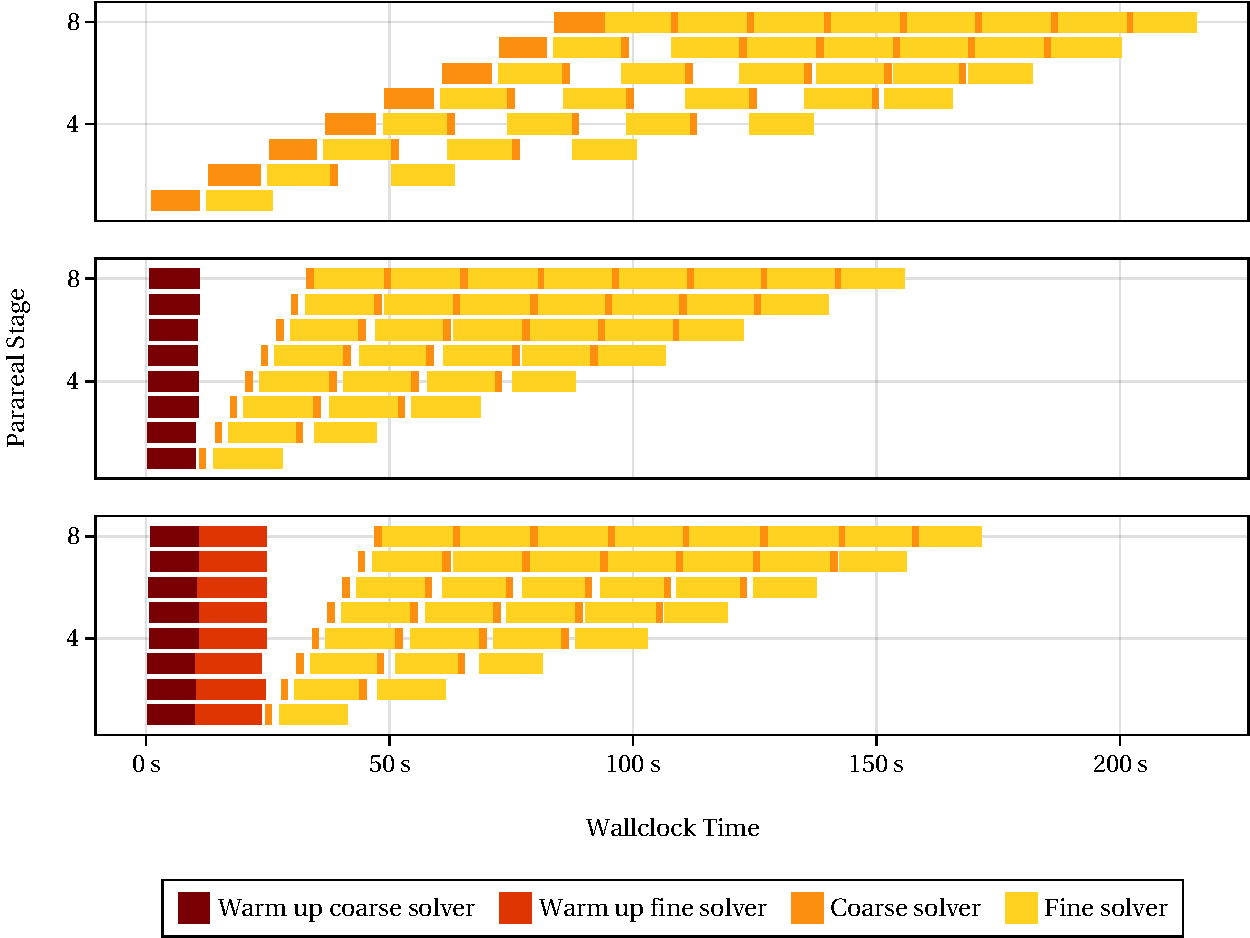
\includegraphics[width=\textwidth]{figures/fig_impl_warmup1.pdf}%
    \renewcommand\thefigure{7.1} % number in thesis
    \caption{Timeline charts}
    \lstinline!bash fig:impl:warmup.job!
    \end{figure}
  \column{0.35\textwidth}
    \begin{itemize}
      \item
        No warm-up:\\ sequential compilation
        \vspace{2em}
      \item
        Warming-up $G$:\\ parallel compilation
        \vspace{2em}
      \item
        Warming-up $F,G$:\\ no further benefit
        \vspace{2em}
      \pause
      \item[$\leadsto$]
        Always warm-up $G$\\ and $G$ only
    \end{itemize}
    \vspace{2em}
  \end{columns}
\end{frame}

\begin{frame}[t]{Estimating Parareal Runtime}
  \begin{block}{Runtime Model}
  %\vspace{-\baselineskip} % maybe needed if in column
  \begin{equation*}
    \hattpar
    := \twarmup
    + \underbrace{
      \strut
      N \cdot (\trampup + t_G)
    }_{\substack{
      \text{stages $1\leq n\leq N$}\\
      \text{refinement $k=0$}
    }}
    + \underbrace{
      \strut
      K \cdot (t_F + t_G)
    }_{\substack{
      \vphantom{\text{stage}}
      n = N \\
      1 \leq k \leq K
    }}
    + t_F
  \end{equation*}
  \end{block}
  \only<1>{%
  \begin{columns}[onlytextwidth]
  \column{0.7\textwidth}
  \begin{figure}
    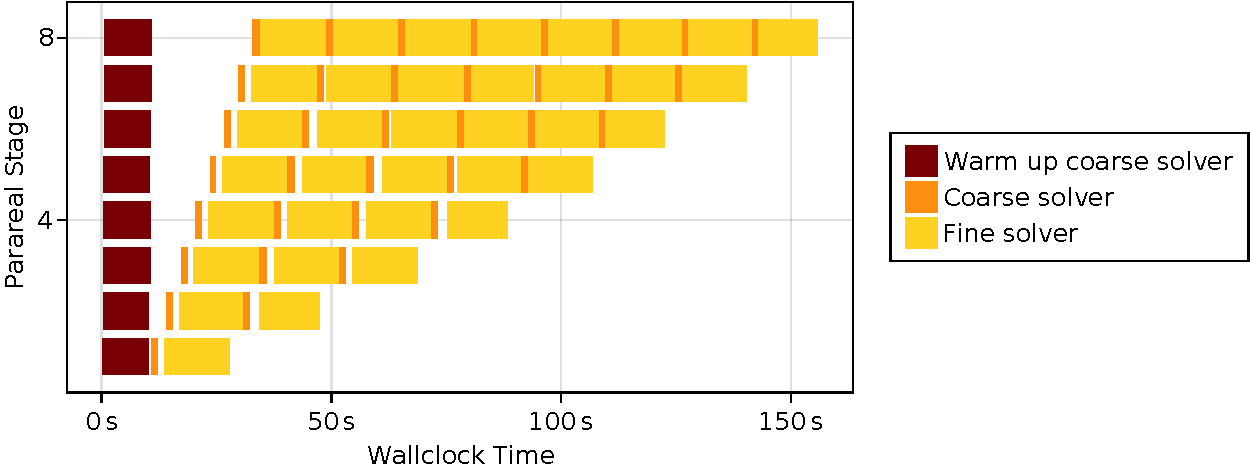
\includegraphics[width=\textwidth]{figures/slides_timeline8.pdf}
    \caption{Timeline of $N=8$ stages computing $K=7$ refinements}
  \end{figure}
  \column{0.32\textwidth}
  \begin{itemize}
    \item under suitable assumptions
    \item $t_G/t_F$: runtime of coarse/fine solver
    \item $\twarmup$: duration of warm-up %TODO: is this really needed?
    \item $\trampup$: delay between first coarse solves
  \end{itemize}
  \end{columns}
  }
  \only<2>{%
  \setbeamertemplate{caption}[numbered]
  \vspace{-\baselineskip}
  \begin{table}
    \renewcommand\thetable{7.1} % number in thesis
    \caption{Runtime measurements for dense Rail371. (timings in seconds)}
    \small
    \begin{tabular}{%
      lcc
      S[table-format=2.2]
      S[table-format=2.2]
      S[table-format=1.2]
      S[table-format=2.2]
      S[table-format=3.2]
      S[table-format=3.2]
      S[round-precision=3, round-minimum=0.001, table-format=<1.3, scientific-notation=fixed, fixed-exponent=0] % err
    }
      \toprule
      {warm-up} &
      {$N$} &
      {$K$} &
      {$\twarmup$} &
      {$\trampup$} &
      {$t_G$} &
      {$t_F$} &
      {$\tpar$} &
      {$\hattpar$} &
      {$\abs*{\frac{\hattpar-\tpar}{\tpar}}$} \\
      \midrule
      none & 8 & 7 & 0.0 & 10.448182003838676 & 1.3971984386444092 & 13.686557531356812 & 215.85136604309082 & 214.03589286123002 & -0.008410756045427896 \\
$G$ & 8 & 7 & 10.995897054672241 & 1.7753152676991055 & 1.3795734643936157 & 14.053897976875305 & 155.979896068573 & 158.32320497717177 & 0.015023147005871765 \\
$G$ and $F$ & 8 & 7 & 24.658120155334473 & 1.805815781865801 & 1.3864995241165161 & 13.99841558933258 & 171.88022804260254 & 171.88946398666928 & 5.373476735471789e-5 \\

      \bottomrule
    \end{tabular}
  \end{table}
  %\vspace{-\baselineskip}
  \begin{columns}[t,onlytextwidth]
  \column{0.285\textwidth}
  \begin{itemize}
    \item $\twarmup$: maximum
    \item $t_F,t_G$: median
  \end{itemize}
  \column{0.4\textwidth}
  \begin{itemize}
    \item $\trampup$: mean dealy between\\ first coarse solves minus $t_G$
  \end{itemize}
  \column{0.3\textwidth}
  \begin{itemize}
    \item actual runtime $\tpar$:\\ end of last fine solve
  \end{itemize}
  \end{columns}
  }
\end{frame}


\section{Results}

\subsection{Numerical Results}

\begin{frame}[label=other]{\secname}
\framesubtitle{\subsecname}
  \setbeamertemplate{caption}[numbered]
  \begin{columns}[onlytextwidth]
  \column{0.7\textwidth}
  \begin{minipage}[b][0.75\textwidth][c]{\textwidth}
  \setlength{\belowcaptionskip}{0pt}
\only<+>{
  \begin{figure}
  \renewcommand\thefigure{7.7} % number in thesis
  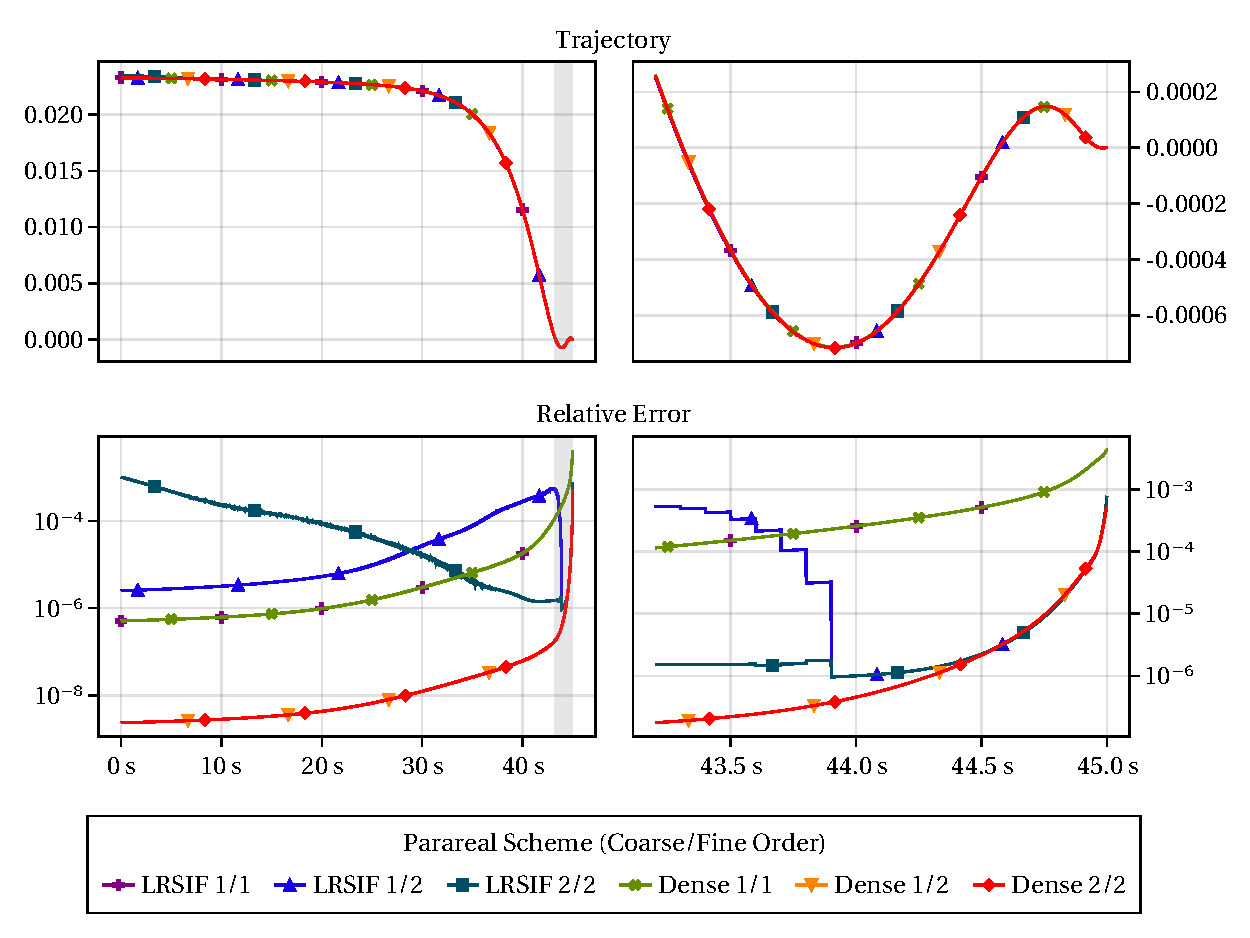
\includegraphics[width=0.9\textwidth]{figures/fig_results_parareal.pdf}%
  \caption{Trajectory $X_{1,77}$ and relative error in $K$ for Rail371}
  \label{fig:7.7}
  \end{figure}
}
\only<+>{
  \begin{figure}
  \renewcommand\thefigure{7.8} % number in thesis
  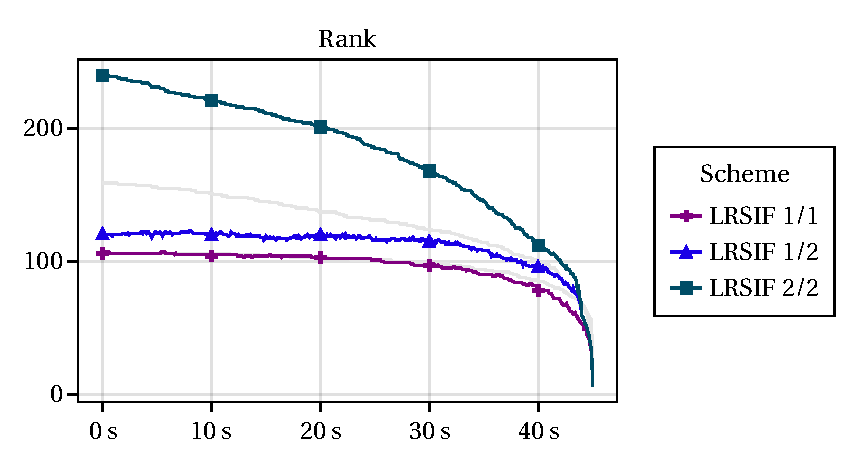
\includegraphics[width=0.9\textwidth]{figures/fig_results_parareal_rank.pdf}%
  \caption{Rank of $X=LDL^\T$ for Rail371}
  \end{figure}
}
\only<+>{
  \begin{figure}
  \renewcommand\thefigure{7.9} % number in thesis
  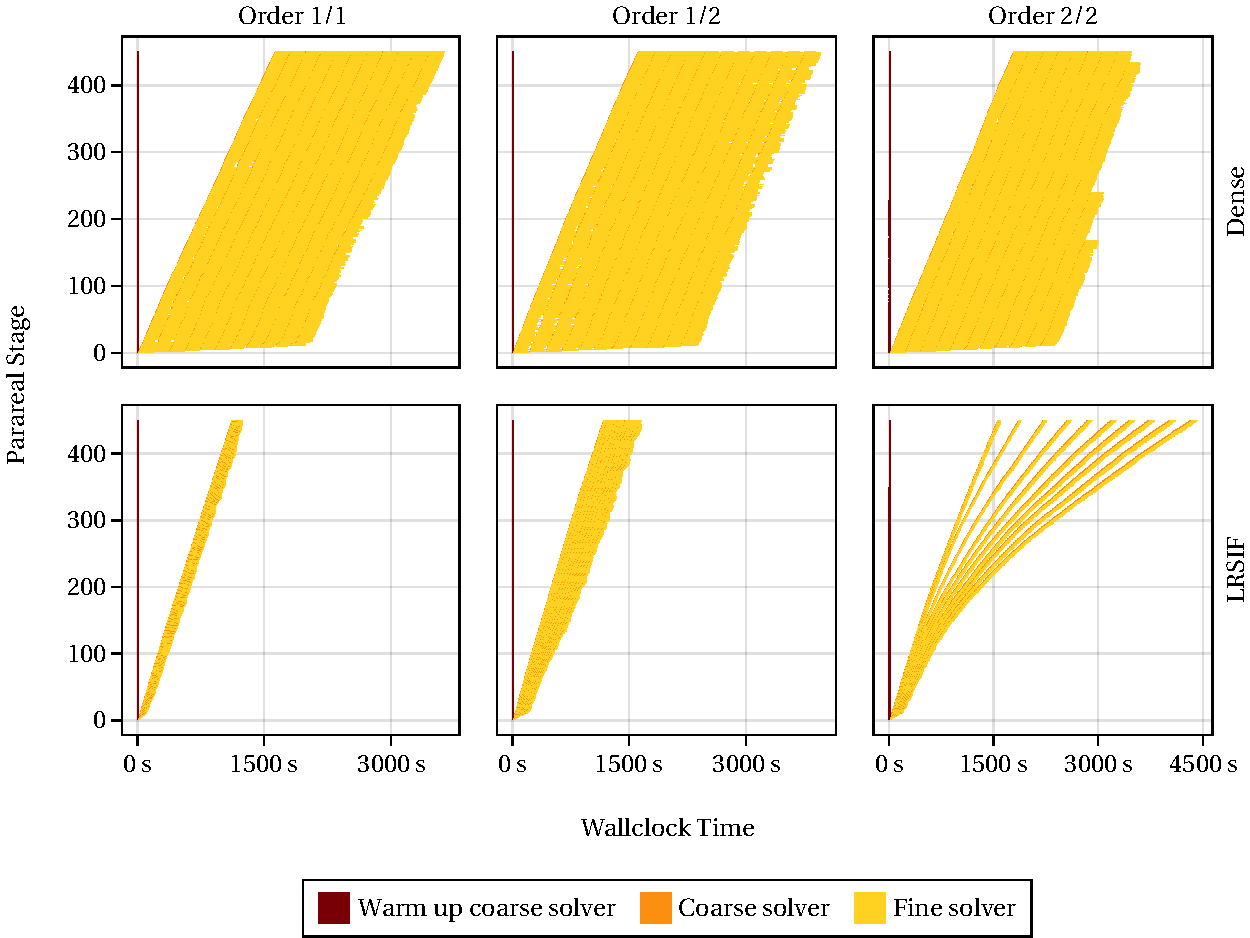
\includegraphics[width=0.85\textwidth]{figures/fig_timeline_all.pdf}%
  \caption{Timeline chart of parareal method applied to Rail371}
  \end{figure}
}
  \end{minipage}
  \column{0.3\textwidth}
  \begin{block}{Parareal Setup}
    \begin{itemize}
      \item
        450 coarse steps (\SI{100}{\milli\second})
      \item
        100 fine steps per coarse step (\SI{1}{\milli\second})
      \item
        Max.~\#iterations: 10
      \item
        Convergence:\\
        relative change in~$X$\\ below $371\umach$,\\
        twice in a row,\\
        max.~1 iteration\\
        behind prev.~stage,\\
        and all previous\\
        stages converged
    \end{itemize}
  \end{block}
  \end{columns}
\end{frame}

\subsection{Parallel Scaling}

\begin{frame}[b,fragile,label=speedup]{\secname}
\framesubtitle{\subsecname}
  \setbeamertemplate{caption}[numbered]
  \begin{columns}[c,onlytextwidth]
  \column{0.65\textwidth}
  \begin{table}
  \setlength{\abovecaptionskip}{0pt}
  %TODO: use hanging captions
  \raggedright
  \renewcommand\thetable{7.3} % number in thesis
  \caption{%
    Speed-up and parallel efficiency of parareal method applied to Rail371 using $N=450$ cores.
    (timings in seconds)
  }
  \begin{tabular}{%
    l
    S[table-format=4.2] % par
    S[table-format=6.2] % seq est
    S[table-format=2.2] % speedup
    S[round-precision=3, round-minimum=0.001, table-format=1.3, table-space-text-post=$^{*}$] % efficiency
  }
    \toprule
    Solver &
    {$\tpar$} &
    {$\hattseq$} &
    {$\frac{\hattseq}{\tpar}$} &
    {$\frac{\hattseq}{N\cdot\tpar}$} \\
    \midrule
    LRSIF 1/1 & 1243.838875055313 & 4313.1015791893005 & 3.4675725816959195 & 0.007705716848213155 \\
LRSIF 1/2 & 1659.4842681884766 & 14054.911208629608 & 8.469445283727943 & 0.018820989519395426 \\
LRSIF 2/2 & 4417.833864927292 & 24565.040289878845 & 5.560426453538251 & 0.012356503230085001 \\

    \addlinespace
    Dense 1/1 & 3627.2994508743286 & 75037.70862150192 & 20.686935180776086 & 0.0459709670683913 \\
Dense 1/2 & 3956.8617849349976 & 84595.60539913177 & 21.379469386879656 & 0.04750993197084368 \\
Dense 2/2 & 3602.3622279167175 & 89274.93912768364 & 24.78233266933632 & 0.05507185037630293 \\

    \addlinespace
    Dense 4/4 & 3381.8760890960693 & 115091.05863285065 & 34.03171955469633 & 0.07562604345488073 \\

    \midrule
    \pause
    Rail1357 & 3001.4058759212494 & 22684.368317604065 & 7.557914275969537 & 0.016795365057710083$^{*}$ \\
    \bottomrule
  \end{tabular}
  \end{table}
  \column{0.35\textwidth}
  \begin{block}{Addendum}
  \begin{itemize}
    \item
      Actual runtime of (sequential) Dense 4:

      $\tseq < \SI{86831}{\second}$

      (Slurm job duration)
    \item
      LRSIF 1/1 applied to Rail1357:
      % TODO: goto button for timeline (and back button there)

      \begin{itemize}
        \item
          2 BLAS threads\\ per process
        \item
          $2\times$ round-robin scheduling onto\\
          $P=225$ processes
        \item[{\makebox[\widthof{\usebeamertemplate{itemize item}}][c]{$\ast$}}]
          actual efficiency:
          $2\hattseq/2P\cdot \tpar = \num[round-precision=3]{0.033590730115420166}$
      \end{itemize}

      % $\tpar = \SI{3600}{\second}$ (Slurm job duration)
  \end{itemize}
  \end{block}
  {\hfill\hyperlink{app:rail1357}{\beamergotobutton{Appendix}}}
  \vspace{-\baselineskip}
  \end{columns}
  \onslide
  \vfill
  \begin{lstlisting}
MY_KIND=dense MY_NF=100 MY_OF=1 MY_OC=1 sbatch -n450 -J de11 par.job
  \end{lstlisting}
\end{frame}

\subsection{Conclusion}

\begin{frame}<1>[label=conclusion]{\secname}
\framesubtitle{\subsecname}
\begin{block}{Parareal Method}
  \begin{itemize}
    \item
      Offers large speed-ups, but has low efficiency
    \item
      Present implementation has severe ramp-up delay

      \uncover<2>{due to Julia's JIT compiler warm-up}
    \item
      Low-rank codes allow/require much smaller (temporal) resolutions

      \uncover<2>{to reach similar speed-ups as dense codes}
    \item
      Runtime of low-rank solvers varies from evaluation to evaluation

      \uncover<2>{due to varying rank and stiffness}
      $\leadsto$ complicates load balancing
  \end{itemize}
\end{block}
\begin{block}{DRE Solvers}
  \begin{itemize}
    \item
      Ros1 performs identically for dense and low-rank data
    \item
      Reproduced issues with low-rank Ros2 in Julia

      \uncover<2>{\cite{Lang2015} had used MATLAB}
  \end{itemize}
\end{block}
\end{frame}

\begin{frame}<1>[label=conclusion]{\secname}
\framesubtitle{Open Problems}
\begin{block}{ParaReal.jl}
  \begin{itemize}
    \item
      Currently limited to processes as executors
    \item
      Lacks asynchronous communication
    \item
      How to eliminate the ramp-up delay?

      \uncover<2>{\ie compile more code ahead-of-time}
    \item
      How to improve load balancing?

      \uncover<2>{%
      \eg via round-robin scheduling or threaded oversubscription;\\
      but how to handle threads \& processes?
      }
  \end{itemize}
\end{block}
\begin{block}{DifferentialRiccatiEquations.jl}
  \begin{itemize}
    \item
      Needs to record more metrics
    \item
      \texttt{\LDLt} (and \texttt{LowRankUpdate}) types could be separated into their own packages
  \end{itemize}
\end{block}
\end{frame}


\section{Summary}

\begin{frame}
  \frametitle{Summary}
  foo
\end{frame}

\appendix

\documentclass[
  aspectratio=1610,
]{beamer}

%\includeonlyframes{current,other}

\usepackage[american]{babel}
\usepackage[utf8]{inputenc}
\usepackage[T1]{fontenc}

% needs https://tex.stackexchange.com/questions/423848/xelatex-xy-and-dejavu-otf#423854
%\usepackage{dejavu-otf} % default Makie font: DejaVu Sans
%\usefonttheme{professionalfonts}

\title{A Low-Rank Parareal Solver for\\ Differential Riccati Equations\\ Written in Julia}
\author{Jonas Schulze}
\institute{Faculty of Mathematics\\ Otto-von-Guericke-Universität Magdeburg}
\date{May 10, 2022}
\subject{subject}

% beamer appearance
\setbeamercolor{block body}{bg=mpi} % for debugging
\setbeamercovered{transparent}
\beamertemplatenavigationsymbolsempty

\newcommand\maketocframe[1][]{%
  \begin{frame}{Outline}
    \tableofcontents[#1]
  \end{frame}
}

\AtBeginSection{%
  \maketocframe[currentsection,currentsubsection]
}

\usepackage[
  style=authoryear,
]{biblatex}
\addbibresource{stuff.bib}

\usepackage{mathtools}
\usepackage{xparse,xspace}
\usepackage{booktabs}
\usepackage{csquotes}
\usepackage[shortcuts]{glossaries}
\usepackage[binary-units]{siunitx}
\usepackage{listings}

\lstset{
  basicstyle=\small\ttfamily\color{black!15}, % should match transparency of covered
  columns=flexible,
}

\usepackage{tikz}
\usetikzlibrary{positioning}
\usetikzlibrary{graphs,arrows.meta}
\tikzset{>=Stealth}

\sisetup{
  round-mode = places,
  round-precision = 2,
}

\newcommand{\N}{\mathbb{N}} % Natural numbers
\newcommand{\Z}{\mathbb{Z}} % Whole numbers
\newcommand{\Q}{\mathbb{Q}} % Rational numbers
\newcommand{\R}{\mathbb{R}} % Real numbers
\newcommand{\C}{\mathbb{C}} % Complex numbers
\newcommand{\F}{\mathbb{F}} % Arbitrary Field
\newcommand{\K}{\mathbb{K}} % Arbitrary Field

\newcommand{\Cneg}{\C_-} % Negative Half Plane

\newcommand{\im}{i} % imaginary unit

\newcommand{\onehalf}{\tfrac{1}{2}}

% matrices
\newcommand\Cnn{\C^{n\times n}}
\newcommand\Rnn{\R^{n\times n}}
\newcommand\Rnr{\R^{n\times r}}
\newcommand\Rnk{\R^{n\times k}}
\newcommand\Rkk{\R^{k\times k}}
\newcommand\nnz{\operatorname{nnz}}
\renewcommand\vec{\operatorname{vec}}
\DeclareMathOperator{\colspan}{span}
\DeclareMathOperator{\orth}{orth}
\DeclareMathOperator{\rank}{rank}
\DeclareMathOperator{\diag}{diag}
\newcommand\MP{\dagger} % Moore Penrose pseudo-inverse

% transpose and conjugate/Hermitian transpose:
\newcommand\conj[1]{\overline{\optional{#1}}}
\newcommand\T{T}
\newcommand\HT{H}

% Rosenbrock
\newcommand\Ham{\ensuremath{H}}
\newcommand\Ricc{\operatorname{\mathcal R}}
\newcommand\Jac{\operatorname{\mathcal J}}

 % ADI
\newcommand\Aip{\mathop{H_k^+}}
\newcommand\Aim{\mathop{H_k^-}}
\newcommand\Aipm{\mathop{H_k^\pm}}
\newcommand\Aiip{\mathop{V_k^+}}
\newcommand\Aiim{\mathop{V_k^-}}
\newcommand\Aiipm{\mathop{V_k^\pm}}
\newcommand\Cayley{\mathop{\mathcal{C}}}
\newcommand\Aipinv{\mathop{(\Aip)^{-1}}}
\newcommand\Aiipinv{\mathop{(\Aiip)^{-1}}}
\newcommand\Lyap{\operatorname{\mathcal L}}

% usage: \{2x\given x\in\N}
\newcommand{\given}{\mid}

% usage: \Set[\big]{2x \given x\in\N}
\newcommand\SetSymbol[1][]{%
  \nonscript\:#1\vert
  \allowbreak
  \nonscript\:
  \mathopen{}}
\DeclarePairedDelimiterX{\Set}[1]{\lbrace}{\rbrace}{%
  \renewcommand\given{\SetSymbol[\delimsize]}% this effect is local only
  #1%
}

% personal taste:
\let\epsilon\varepsilon
%\renewcommand{\to}{\longrightarrow}
%\renewcommand{\mapsto}{\longmapsto}
%\renewcommand{\gets}{\longleftarrow}
\renewcommand{\Re}{\operatorname{Re}} % real part of a complex number
\renewcommand{\Im}{\operatorname{Im}} % imaginary part

% some more delimiters:
\NewDocumentCommand{\optional}{m}{\ifblank{#1}{\,\cdot\,}{#1}}
\DeclarePairedDelimiterX{\abs}[1]{\lvert}{\rvert}{\optional{#1}}
\DeclarePairedDelimiterX{\norm}[1]{\lVert}{\rVert}{\optional{#1}}
\DeclarePairedDelimiterX{\scalar}[2]{\langle}{\rangle}{\optional{#1},\optional{#2}}
\newcommand{\card}{\abs}

% integration:
\NewDocumentCommand{\intd}{m}{\,\textup{d}#1}
\newcommand\dt{\intd{t}}

% differentiation:
\NewDocumentCommand{\pdiff}{mm}{\frac{\partial #2}{\partial #1}}
\NewDocumentCommand{\diff}{mm}{\frac{\mathrm{d} #2}{\mathrm{d} #1}}

\newcommand\julia\texttt
\newcommand\code\texttt

\newcommand\LDLt{LDL\textsuperscript{T}}

\counterwithout*{footnote}{chapter}
\setcounter{topnumber}{1} % max number of floats at top of page
\renewcommand{\bottomfraction}{0.5}
\renewcommand{\listtheoremname}{List of Theorems and Examples}

\newcommand\LandauO{\operatorname{\mathcal O}}

% runtime estimates
\newcommand\hattpar{\hat t_\text{par}} % estimate
\newcommand\hattseq{\hat t_\text{seq}} % estimate
\newcommand\tpar{t_\text{par}}
\newcommand\tseq{t_\text{seq}}
\newcommand\twarmup{t_\text{warm-up}}
\newcommand\trampup{t_\text{ramp-up}}
\newcommand\JIT{\operatorname{compile}}

% error estimates
\newcommand\umach{\mathrm u_\text{mach}} % machine precision

% https://tex.stackexchange.com/questions/22561/what-is-the-proper-use-of-i-e-backslash-at?noredirect=1&lq=1
\makeatletter % no idea why this is needed. \@ifnextchar doesn't work without it.
\newcommand\cf{cf.\@\xspace} % confer
\newcommand\eg{e.g.\@\xspace} % exempli gratia
\newcommand\etc{etc\@ifnextchar.{}{.\@\xspace}} % et cetera
\newcommand\ie{i.e.\@\xspace} % id est
\newcommand\wrt{w.r.t.\@\xspace} % with respect to
\makeatother

\definecolor{mathcore} {RGB}{102,  99, 100}
\definecolor{ovgu math}{RGB}{209,  63,  88}
\definecolor{mpi}      {RGB}{ 61, 167, 197}
\def\cola{ovgu math}
\def\colb{mathcore}
\def\colc{mpi}

\tikzset{
  mat/.style={
    rectangle,
    minimum size=1ex,
    inner sep=0mm,
  },
  bigmat/.style={mat,minimum size=#1},
  bigmat/.default=1cm,
  tallmat/.style={mat,minimum height=#1},
  tallmat/.default=1cm,
  widemat/.style={mat,minimum width=#1},
  widemat/.default=1cm,
  smallmat/.style={mat},
}

\newcommand\mat[2]{%
  \tikz[baseline=(M.base)] \node [mat, #1, fill=ovgu math] (M) {$#2$};
}
\newcommand\bigmat[1]{\mat{minimum size=2cm}{#1}}
\newcommand\tallmat[2][6mm]{\mat{minimum size=#1, minimum height=2cm}{#2}}
\newcommand\widemat[2][6mm]{\mat{minimum size=#1, minimum width=2cm}{#2}}
\newcommand\smallmat[2][6mm]{\mat{minimum size=#1}{#2}}

\newcommand\tallcmat[1]{\tikz[baseline=-0.5ex]\node[tallmat,fill=#1] {};}
\newcommand\smallcmat[1]{\tikz\node[smallmat,fill=#1] {};}
\newcommand\widecmat[1]{\tikz\node[widemat,fill=#1] {};}
\newcommand\colorldlt[1]{%
  \mathop{\tallcmat{#1}}
  \mathop{\smallcmat{#1}}
  \mathop{\widecmat{#1}}
}

\newcommand\colorspacing{%
  \arraycolsep=3pt
  \def\arraystretch{0.75}
}


\renewcommand\mathrm\mathsf % fix \umach
\newcommand\emptyblock[1]{%
  \begin{beamercolorbox}{block title}
    \usebeamerfont{block title}%
    #1
  \end{beamercolorbox}
}

%TODO: what if the frame needs multiple slides?
\newcommand\bigpicture[1]{%
  \begin{block}{Big Picture}
    \begin{itemize}
      \item
        Differential \Riccati Equation (DRE)
      \ifnum#1<2 \pause\fi
      \item
        Solution in LRSIF
      \ifnum#1<3 \pause\fi
      \item
        Rosenbrock method\\ to solve DRE
      \ifnum#1<4 \pause\fi
      \item
        Rosenbrock stages are ALEs
      \ifnum#1<5 \pause\fi
      \item
        ADI method\\ to solve ALE
      \ifnum#1<6 \pause\fi
      \item
        Parareal method\\ for speed-up
    \end{itemize}
  \end{block}
}

\newcommand\tallcmat[1]{\tikz[baseline=-0.5ex]\node[tallmat,fill=#1] {};}
\newcommand\smallcmat[1]{\tikz\node[smallmat,fill=#1] {};}
\newcommand\widecmat[1]{\tikz\node[widemat,fill=#1] {};}
\newcommand\colorldlt[1]{%
  \mathop{\tallcmat{#1}}
  \mathop{\smallcmat{#1}}
  \mathop{\widecmat{#1}}
}

\newcommand\colorspacing{%
  \arraycolsep=3pt
  \def\arraystretch{0.75}
}

\begin{document}

\frame[plain]{\titlepage}
\maketocframe

\everymath{\displaystyle}

\section{Motivation}

\begin{frame}{Motivation}
  \begin{columns}[t,onlytextwidth]
  \column{0.5\linewidth}
  \begin{block}{\strut Optimal Control Problem}
    Consider the \acf{LQR} problem
    \begin{equation*}
      \begin{array}{cl}
        \min_u & \int_{t_0}^{t_f} y^\T y + u^\T u \dt + \tfrac{1}{100} y(t_f)^\T y(t_f) \medskip\\
        \text{s.t.} & \begin{aligned}[t]
          E \dot x &= Ax + Bu \\
          y &= Cx
        \end{aligned}
      \end{array}
    \end{equation*}
    using
    \begin{itemize}
      \item
        state $x(t)\in\R^n$
      \item
        control $u(t)\in\R^m$, $m\ll n$
      \item
        output $y(t)\in\R^q$, $q\ll n$
      \item
        constant system matrices $E,A,B,C$.
    \end{itemize}
  \end{block}
  \pause
  \column{0.47\linewidth}
  \begin{block}{\strut Feedback Law \parencite[e.g.][]{Locatelli2011}}
    The optimal control is given by
    \begin{equation*}
      u(t) = -
        B^\T X(t_f+t_0-t) E
      x(t)
    \end{equation*}
    where $X(t)\in\R^{n\times n}$ solves the \acf{DRE}
    \begin{equation*}
      \left\{
        \begin{lgathered}
          E\dot X E = \begin{multlined}[t]
            C^\T C + A^\T X E + E^\T X A \\ - E^\T X BB^\T X E
          \end{multlined} \\
          E^\T X(t_0) E = \tfrac{1}{100} C^\T C
          .
        \end{lgathered}
      \right.
    \end{equation*}
  \end{block}
  \end{columns}
\end{frame}

\begin{frame}{Oberwolfach Rail}
\begin{columns}[onlytextwidth]
\column{0.6\textwidth}
  \begin{itemize}
    \item
      \cite{Benner2005}
    \item
      Linearized 2D heat equation:
      \begin{align*}
        c \rho\, \partial_t x &= \lambda\,\Delta x, && x\in\Omega\\
        \lambda\, \partial_n x &= q_k (u_k - x), && x \in\Gamma_k, k=1,\ldots,7\\
        \partial_n x &= 0, && x\in\Gamma_0
      \end{align*}
    \item
      FEM discretizations / mesh refinements with
      $n\in\Set{371,1357,5177,\num{20209},\ldots}$ states,\\
      $m=7$ inputs,
      $q=6$ outputs
    \item
      Time horizon $t\in[\SI{0}{\second}, \SI{45}{\second}]$
    \item
      Resulting $(E, A, B, C)$ system:
      $E \succ 0$ and $A \prec 0$\\
      $\leadsto$ uniquely solvable
  \end{itemize}
\column{0.37\textwidth}
  \includegraphics[width=\textwidth]{figures/Steelprofile1.jpg}
\end{columns}
\end{frame}

\begin{frame}<1>{Motivation}
\begin{bigpicturecols}
  \begin{itemize}
    \item
      Large-scale problems: a single (dense) $X(t)\in\Rnn$\\
      takes \SI{200}{\tera\byte} for
      $n=\num{5000000}$
    \item
      Solution $X$ is symmetric and dense, but has low rank

      \parencite[e.g.][]{Penzl2000}
    \item[$\leadsto$]
      Approximation via \rlap{\acl{LRSIF}:}
      \begin{equation*}
        \bigmat{X} \approx \mathop{\tallmat{L}} \mathop{\smallmat{D}} \mathop{\widemat{L^{\smash{\T}}}}
      \end{equation*}
    \item
      DRE is highly stiff, \ie\\
      high accuracy requires small time steps or high orders
    \item[$\leadsto$]
      Parareal method for speed-up
  \end{itemize}
\column{\bigpicturewidth}
\bigpicture{1}
\end{bigpicturecols}
\end{frame}


\section{Next}

\subsection{Low-Rank Symmetric Indefinite Factorization}

\begin{frame}<1>{Low-Rank Symmetric Indefinite Factorization (LRSIF)}
\begin{bigpicturecols}
  \begin{itemize}
    \item
      \cite{Benner2009}
    \item
      Arithmetic:
      \begin{equation*}
        \colorspacing
        \colorldlt{\cola} \pm \colorldlt{\colc}
        :=
        \Bigg[
        \begin{matrix}
          \tallcmat{\cola} &
          \tallcmat{\colc}
        \end{matrix}
        \Bigg]
        \begin{bmatrix}
          \smallcmat{\cola} \\
          & \pm \smallcmat{\colc}
        \end{bmatrix}
        % flag of the Netherlands:
        \begin{bmatrix}
          \widecmat{\cola} \\
          \widecmat{\colc}
        \end{bmatrix}
      \end{equation*}
    \item
      Problem: growing storage requirements, \eg
      \begin{equation*}
        \colorspacing
        \colorldlt{\cola} + \colorldlt{\cola}
        :=
        \Bigg[
        \begin{matrix}
          \tallcmat{\cola} &
          \tallcmat{\cola}
        \end{matrix}
        \Bigg]
        \begin{bmatrix}
          \smallcmat{\cola} \\
          & \smallcmat{\cola}
        \end{bmatrix}
        % flag of Austria:
        \begin{bmatrix}
          \widecmat{\cola} \\
          \widecmat{\cola}
        \end{bmatrix}
        %\not\equiv
        %\mathop{\tallcmat{\cola}}
        %\mathop{(\smallcmat{\cola} + \smallcmat{\cola})}
        %\mathop{\widecmat{\cola}}
      \end{equation*}
      $\leadsto$ compression necessary
      (how: \cite{Lang2017})
    \item
      Note: \enquote{low-rank} versions of a matrix or algorithm refer to \enquote{LRSIF}
  \end{itemize}
\column{\bigpicturewidth}
\bigpicture{2}
\end{bigpicturecols}
\end{frame}

\subsection{Rosenbrock Method}

\begin{frame}<1>{Rosenbrock Method}
\begin{columns}
\column{0.7\textwidth}
  \begin{block}{General Formulation}
    For the initial value problem (IVP) $\dot x = f(x)$ the method reads
    \begin{equation*}
    \left\{
    \begin{aligned}
      x_{n+1} &:= x_n + \tau \sum_{j=1}^s b_j k_j
      \\
      k_i &:= \begin{multlined}[t]
      f\left( x_n + \tau \sum_{j=1}^{i-1} \alpha_{ij} k_j \right) + \tau \Jac \sum_{j=1}^i \gamma_{ij} k_j
      \\
      \text{for } i = 1, \ldots, s
      ,
      \end{multlined}
    \end{aligned}
    \right.
    \end{equation*}
    where $\Jac := f'(x_n)$ denotes the Jacobian.
  \end{block}
\column{0.3\textwidth}
\bigpicture{3}
\end{columns}
\end{frame}

\begin{frame}<1>{Rosenbrock Method}
\begin{columns}
\column{0.7\textwidth}
  \begin{block}{1st Order Scheme (Linearly Implicit Euler Scheme)}
    For the IVP $\dot x = f(x)$ the method reads
    \begin{equation*}
    \left\{
    \begin{aligned}
      x_{n+1} &= x_n + \tau k_1 \\
      (I - \gamma\tau \Jac) k_1 &= f(x_n)
      .
    \end{aligned}
    \right.
    \end{equation*}
  \end{block}
  \begin{block}{2nd Order Scheme \parencite{Verwer1999}}
    %\vspace*{-\baselineskip}
    %For the IVP $\dot x = f(x)$ the method reads
    \begin{equation*}
    \left\{
    \begin{aligned}
      x_{n+1} &= x_n + \tfrac{3}{2} \tau k_1 + \tfrac{1}{2} \tau k_2 \\
      (I - \gamma\tau \Jac) k_1 &= f(x_n) \\
      (I - \gamma\tau \Jac) k_2 &= f(x_n + \tau k_1) - 2k_1
    \end{aligned}
    \right.
    \end{equation*}
  \end{block}
\column{0.3\textwidth}
\bigpicture{3}
\end{columns}
\end{frame}

\begin{frame}<-4>{Rosenbrock Method}
\begin{columns}
\column{0.7\textwidth}
\begin{itemize}
\item
  Consider the DRE $E^\T \dot X E = \Ricc(X)$.
  \newcommand\U{\alert{\makebox[\widthof{$X_n$}]{$U$}}}
  \begin{align*}
    \Ricc(X_n) &= C^\T C + A^\T X_n E + E^\T X_n A - E^\T X_n BB^\T X_n E
    \\
    \pause
    \Jac(\alert{U}) &= \makebox[\widthof{$C^\T C$}]{$0$}
      + A^\T \U E + E^\T \U A
      \begin{lgathered}[t]
        {} - E^\T \U BB^\T X_n E \\
        {} - E^\T X_n BB^\T \U E
      \end{lgathered} \\
    \pause
    &= (A - BB^\T X_n E)^\T \alert U E + E^\T \alert U (A - BB^\T X_n E)
  \end{align*}
\item
  The Jacobian is a Lyapunov operator!
\pause
\item %TODO: when \leadsto, when \implies?
  $I - \gamma\tau\Jac$ is a Lyapunov operator,
  \ie all Rosenbrock stages are Algebraic Lyapunov Equations (ALEs).
\end{itemize}
\column{0.3\textwidth}
\bigpicture[3]{3}
\end{columns}
\end{frame}

\begin{frame}<1>{1st Order Rosenbrock Scheme}
\begin{columns}
\column{0.7\textwidth}
  \begin{itemize}
    \item
      Linearly implicit Euler scheme
    \item
      \cite{Mena2007}: Formulation for DRE $E^\T \dot X E = \Ricc(X)$
    \item
      \cite{Lang2017}: Formulation for LRSIF $X(t) = LDL^\T$
    \item
      1 ALE per step:
      \begin{equation*}
        \tilde A_n^\T X_{n+1} E + E^\T X_{n+1} \tilde A_n = - GSG^\T
      \end{equation*}
      where
      \begin{align*}
        \tilde A_n &= \gamma\tau(A-BB^\T X_n E) - \tfrac{1}{2} E
        \\
        G &= \begin{bmatrix}
          C^\T & E^\T L
        \end{bmatrix}
        \\
        S &= \begin{bmatrix}
          I & . \\
          . & DL^\T BB^\T LD + \tfrac{1}{\tau} D
        \end{bmatrix}
      \end{align*}
  \end{itemize}
  \vfill
\column{0.3\textwidth}
\bigpicture{4}
\end{columns}
\end{frame}

\begin{frame}<1>{2nd Order Rosenbrock Scheme}
\begin{columns}
\column{0.7\textwidth}
  \begin{itemize}
    \item
      \cite{Verwer1999}
    \item
      \cite{Mena2007}: Formulation for DRE $E^\T \dot X E = \Ricc(X)$
    \item
      \cite{Lang2017}: Formulation for LRSIF $X(t) = LDL^\T$
    \item
      2 ALEs per step:
      \begin{equation*}
      \left\{
      \begin{aligned}
        X_{n+1} &= X_n + \big( 2 - \tfrac{1}{2\gamma} \big) \tau K_1 - \tfrac{1}{2} \tau K_{21} \\
        \hat A_n^\T K_1 E + E^\T K_1 \hat A_n &= -\Ricc(X_n) \\
        \hat A_n^\T K_{21} E + E^\T K_{21} \hat A_n &= -\big( \tau^2 K_1 BB^\T K_1 + \big( 2-\tfrac{1}{\gamma} \big) K_1 \big)
      \end{aligned}
      \right.
      \end{equation*}
      (LRSIF right-hand sides not shown)
%    \item
%      Embedded 1st order method: $\tilde X_{n+1} = X_n + \gamma\tau K_1$
  \end{itemize}
\column{0.3\textwidth}
\bigpicture{4}
\end{columns}
\end{frame}

\subsection{Parareal Method}

\begin{frame}<-2>{Parareal Method}
\begin{columns}
\column{0.7\textwidth}
  \begin{block}{General Formulation \parencite{Lions2001}}
    For the IVP $\dot u = f(u)$ the method reads
    \begin{equation*}
      \left\{
      \begin{aligned}
        U^0_{n+1} &:= G(U^0_n) \\
        U^{k+1}_{n+1} &:= G(U^{k+1}_n) + F(U^k_n) - G(U^k_n)
      \end{aligned}
      \right.
    \end{equation*}
    where $U_0^0 := u(t_0)$. $U_n^k$ converges to $u(t_n)$ as $k\to\infty$.
  \end{block}
  \begin{itemize}
    \item
      Köhler, Saak, and Lang 2016:
      LRSIF formulation
  % GAMM Annual Meeting
  \begin{equation*}
    U^{k+1}_{n+1}
    =\vphantom{\Bigg[}\parbox{6cm}{$%
    \alt<1>{
      \colorldlt{\cola}
    + \colorldlt{\colb}
    - \colorldlt{\colc}
    }{
    \colorspacing % must be located in respective cell!
    \Bigg[
    \begin{matrix}
      \tallcmat{\cola} &
      \tallcmat{\colb} &
      \tallcmat{\colc}
    \end{matrix}
    \Bigg]
    \begin{bmatrix}
      \smallcmat{\cola} \\
      & \smallcmat{\colb} \\
      && -\smallcmat{\colc}
    \end{bmatrix}
    \begin{bmatrix}
      \widecmat{\cola} \\
      \widecmat{\colb} \\
      \widecmat{\colc}
    \end{bmatrix}
    }$}
  \end{equation*}
    \item
      Speed-up $\approx t_F/t_G$ for large $N$,
      where $0 \leq n \leq N$
  \end{itemize}
\column{0.3\textwidth}
\bigpicture{6}
\end{columns}
\end{frame}

%TODO: replace caption by parareal update formula?
\begin{frame}
  \setbeamertemplate{caption}[numbered]
  \frametitle{Parareal Example}
\begin{columns}
\column{0.65\textwidth}
  \begin{figure}
  \foreach \k in {0,1} {%
  \foreach \n [evaluate={\i=int(1+\n+\k*7)}] in {0,...,6} {%
    \includegraphics<\i>[width=\textwidth]{figures/parareal-anim/step-\k-\n.pdf}%
  }}%
  \includegraphics<15>[width=\textwidth]{figures/parareal-anim/step-2-5.pdf}%
  \includegraphics<16>[width=\textwidth]{figures/parareal-anim/step-2-6.pdf}%
  \includegraphics<17>[width=\textwidth]{figures/parareal-anim/step-3-5.pdf}%
  \includegraphics<18>[width=\textwidth]{figures/parareal-anim/step-3-6.pdf}%
  \renewcommand\thefigure{6.4} % number in thesis
  \caption{Parareal method applied to a linear ODE}
  \end{figure}
\column{0.35\textwidth}
  %\definecolor{rainbow1}{rgb}{0.5019608f0, 0.0f0, 0.5019608f0}
%\definecolor{rainbow2}{rgb}{0.0f0, 0.0f0, 1.0f0}
%\definecolor{rainbow3}{rgb}{0.0f0, 0.5019608f0, 0.0f0}
%\definecolor{rainbow4}{rgb}{1.0f0, 0.64705884f0, 0.0f0}
%\definecolor{rainbow5}{rgb}{1.0f0, 0.0f0, 0.0f0}

\newcommand\pararealU[2]{\draw (2*#2*\xshift,0) +(\yangle:2*#1*\yshift) node (U#1#2) {$U_{#1}^{#2}$};}
\newcommand\pararealG[2]{\draw (2*#2*\xshift,0) +(\yangle:2*#1*\yshift+\yshift) node (G#1#2) {$G(U_{#1}^{#2})$};}
\newcommand\pararealF[2]{\draw (2*#2*\xshift+\xshift,0) +(\yangle:2*#1*\yshift+\yshift) node (F#1#2) {$F(U_{#1}^{#2})$};}

\begin{tikzpicture}[diag/.style={out=45,in=180}]
  \footnotesize
  \def\xshift{11mm}
  \def\yshift{8mm}
  \def\yangle{90}
  % initial value
  \action<+->{\pararealU{0}{0}}
  % k = 0, coarse solutions
  \foreach \n [evaluate={\nprev=int(\n-1)}] in {1,...,5} {%
  \action<+->{%
    \pararealG{\nprev}{0}
    \pararealU{\n}{0}
    \draw [->] (G\nprev0) -- (U\n0);
    \draw [->] (U\nprev0) -- (G\nprev0);
  }}
  % k = 0, fine solutions
  \action<+->{%
  \foreach \n in {0,...,4} {%
    \pararealF{\n}{0}
    \draw [->] (U\n0) -- (F\n0);
  }}
  % k = 0, transform to ghost
  \action<+->{}
  % k = 1, coarse solutions
  \action<+->{%
  \pararealU{1}{1}
  \draw [->] (F00) -- (U11);
  }
  \foreach \n [evaluate={\nprev=int(\n-1)}] in {2,...,5} {%
  \action<+->{%
    \pararealG{\nprev}{1}
    \pararealU{\n}{1}
    \draw [->] (G\nprev1) -- (U\n1);
    \draw [->] (F\nprev0) -- (U\n1);
    \draw [->] (G\nprev0) to [diag] (U\n1);
    \draw [->] (U\nprev1) -- (G\nprev1);
  }}
  % k = 1, fine solutions
  \action<+->{%
  \foreach \n in {1,...,4} {%
    \pararealF{\n}{1}
    \draw [->] (U\n1) -- (F\n1);
  }}
  % k = 2, coarse solutions
  %\action<+->{%
  %\pararealU{2}{2}
  %\draw [->] (F11) -- (U22);
  %\foreach \n [evaluate={\nprev=int(\n-1)}] in {3,...,5} {%
  %  \pararealG{\nprev}{2}
  %  \pararealU{\n}{2}
  %  \draw [->] (G\nprev2) -- (U\n2);
  %  \draw [->] (F\nprev1) -- (U\n2);
  %  \draw [->] (G\nprev1) to [diag] (U\n2);
  %  \draw [->] (U\nprev2) -- (G\nprev2);
  %}}
  % k = 2, fine solutions
  %\action<+->{%
  %\foreach \n in {2,...,4} {%
  %  \pararealF{\n}{2}
  %  \draw [->] (U\n2) -- (F\n2);
  %}}
  % rest
  \action<+->{%
  \foreach \n in {1,...,4} {%
    \draw (F\n1.north east)+(40:1ex) node [rotate=35] {$\cdots$};
  }}
\end{tikzpicture}

\end{columns}
\end{frame}


\section{Results}

\subsection{Numerical Results}

\begin{frame}[label=other]{\secname}
\framesubtitle{\subsecname}
  \setbeamertemplate{caption}[numbered]
  \begin{columns}[onlytextwidth]
  \column{0.7\textwidth}
  \begin{minipage}[b][0.75\textwidth][c]{\textwidth}
  \setlength{\belowcaptionskip}{0pt}
\only<+>{
  \begin{figure}
  \renewcommand\thefigure{7.7} % number in thesis
  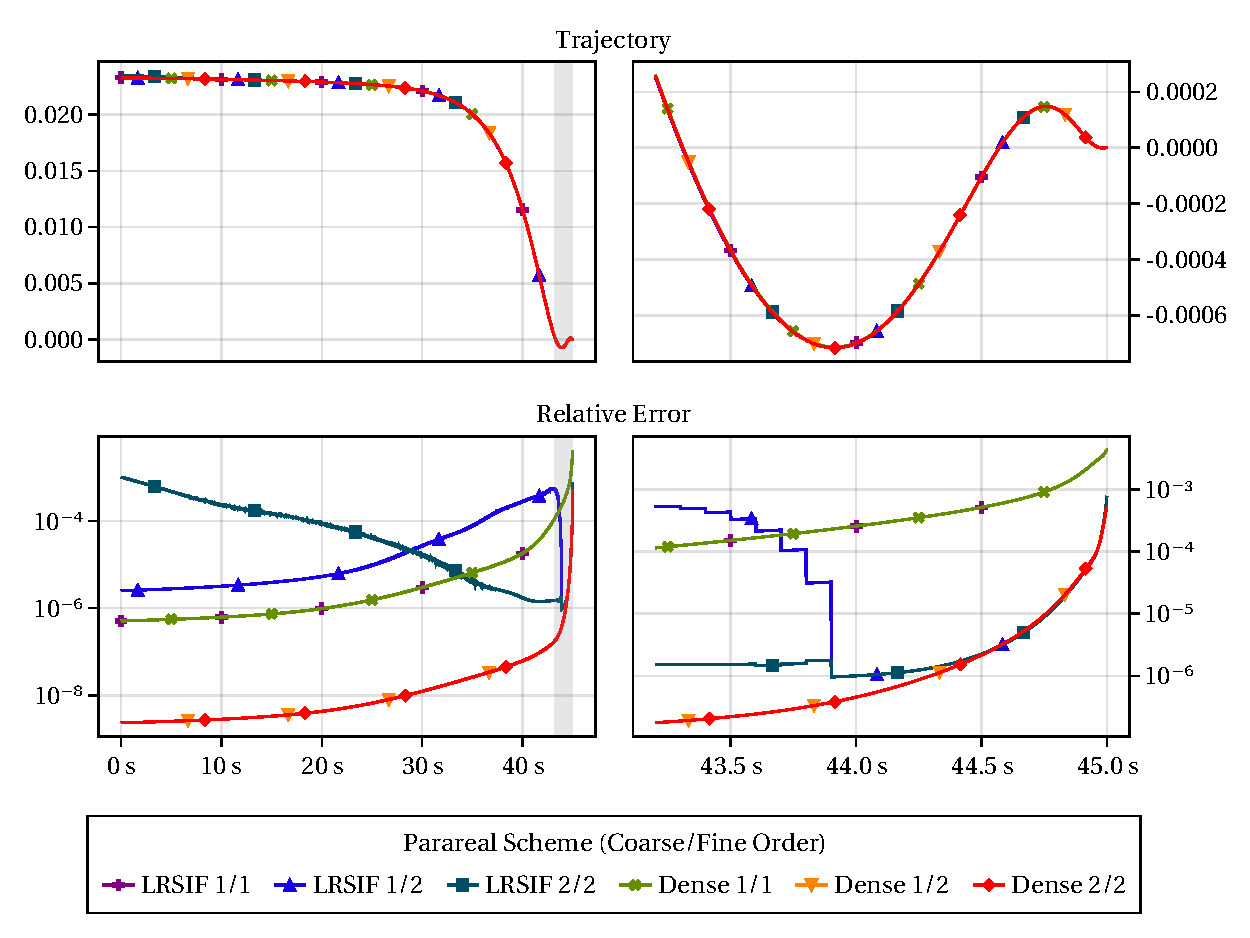
\includegraphics[width=0.9\textwidth]{figures/fig_results_parareal.pdf}%
  \caption{Trajectory $X_{1,77}$ and relative error in $K$ for Rail371}
  \label{fig:7.7}
  \end{figure}
}
\only<+>{
  \begin{figure}
  \renewcommand\thefigure{7.8} % number in thesis
  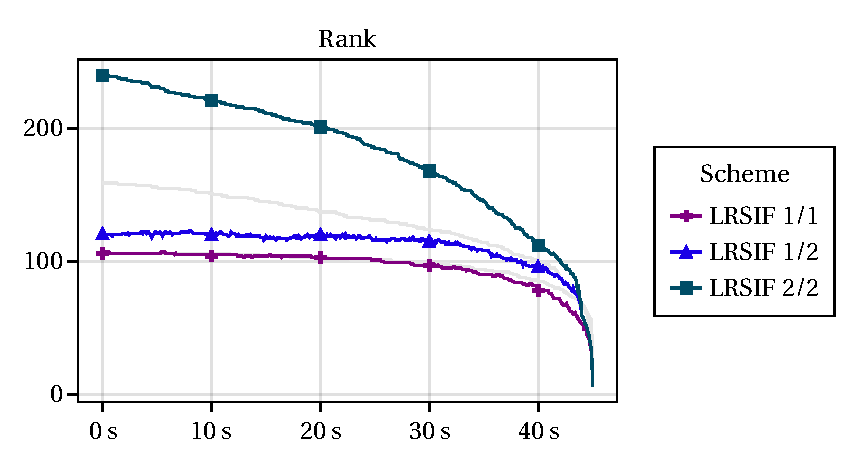
\includegraphics[width=0.9\textwidth]{figures/fig_results_parareal_rank.pdf}%
  \caption{Rank of $X=LDL^\T$ for Rail371}
  \end{figure}
}
\only<+>{
  \begin{figure}
  \renewcommand\thefigure{7.9} % number in thesis
  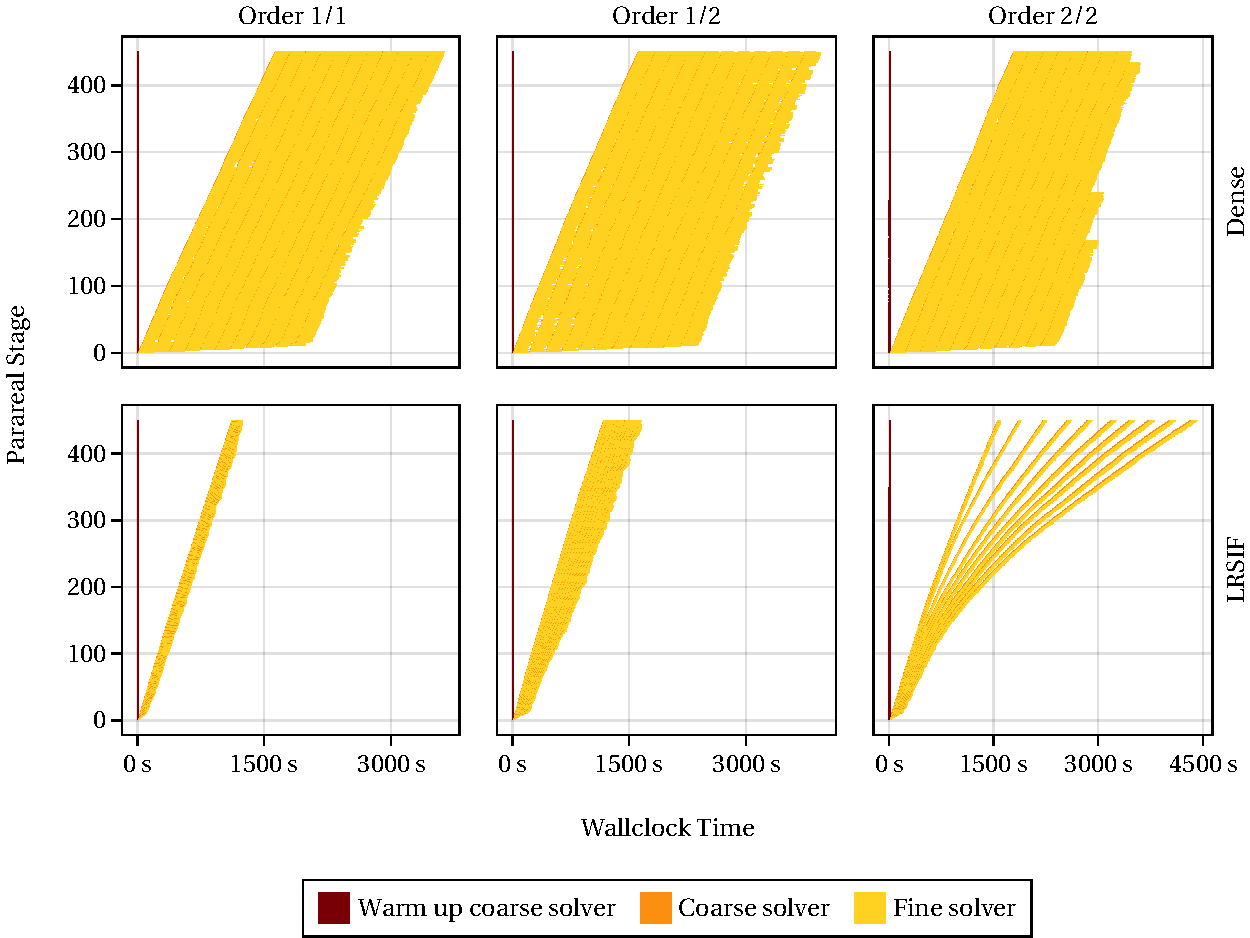
\includegraphics[width=0.85\textwidth]{figures/fig_timeline_all.pdf}%
  \caption{Timeline chart of parareal method applied to Rail371}
  \end{figure}
}
  \end{minipage}
  \column{0.3\textwidth}
  \begin{block}{Parareal Setup}
    \begin{itemize}
      \item
        450 coarse steps (\SI{100}{\milli\second})
      \item
        100 fine steps per coarse step (\SI{1}{\milli\second})
      \item
        Max.~\#iterations: 10
      \item
        Convergence:\\
        relative change in~$X$\\ below $371\umach$,\\
        twice in a row,\\
        max.~1 iteration\\
        behind prev.~stage,\\
        and all previous\\
        stages converged
    \end{itemize}
  \end{block}
  \end{columns}
\end{frame}

\subsection{Parallel Scaling}

\begin{frame}[b,fragile,label=speedup]{\secname}
\framesubtitle{\subsecname}
  \setbeamertemplate{caption}[numbered]
  \begin{columns}[c,onlytextwidth]
  \column{0.65\textwidth}
  \begin{table}
  \setlength{\abovecaptionskip}{0pt}
  %TODO: use hanging captions
  \raggedright
  \renewcommand\thetable{7.3} % number in thesis
  \caption{%
    Speed-up and parallel efficiency of parareal method applied to Rail371 using $N=450$ cores.
    (timings in seconds)
  }
  \begin{tabular}{%
    l
    S[table-format=4.2] % par
    S[table-format=6.2] % seq est
    S[table-format=2.2] % speedup
    S[round-precision=3, round-minimum=0.001, table-format=1.3, table-space-text-post=$^{*}$] % efficiency
  }
    \toprule
    Solver &
    {$\tpar$} &
    {$\hattseq$} &
    {$\frac{\hattseq}{\tpar}$} &
    {$\frac{\hattseq}{N\cdot\tpar}$} \\
    \midrule
    LRSIF 1/1 & 1243.838875055313 & 4313.1015791893005 & 3.4675725816959195 & 0.007705716848213155 \\
LRSIF 1/2 & 1659.4842681884766 & 14054.911208629608 & 8.469445283727943 & 0.018820989519395426 \\
LRSIF 2/2 & 4417.833864927292 & 24565.040289878845 & 5.560426453538251 & 0.012356503230085001 \\

    \addlinespace
    Dense 1/1 & 3627.2994508743286 & 75037.70862150192 & 20.686935180776086 & 0.0459709670683913 \\
Dense 1/2 & 3956.8617849349976 & 84595.60539913177 & 21.379469386879656 & 0.04750993197084368 \\
Dense 2/2 & 3602.3622279167175 & 89274.93912768364 & 24.78233266933632 & 0.05507185037630293 \\

    \addlinespace
    Dense 4/4 & 3381.8760890960693 & 115091.05863285065 & 34.03171955469633 & 0.07562604345488073 \\

    \midrule
    \pause
    Rail1357 & 3001.4058759212494 & 22684.368317604065 & 7.557914275969537 & 0.016795365057710083$^{*}$ \\
    \bottomrule
  \end{tabular}
  \end{table}
  \column{0.35\textwidth}
  \begin{block}{Addendum}
  \begin{itemize}
    \item
      Actual runtime of (sequential) Dense 4:

      $\tseq < \SI{86831}{\second}$

      (Slurm job duration)
    \item
      LRSIF 1/1 applied to Rail1357:
      % TODO: goto button for timeline (and back button there)

      \begin{itemize}
        \item
          2 BLAS threads\\ per process
        \item
          $2\times$ round-robin scheduling onto\\
          $P=225$ processes
        \item[{\makebox[\widthof{\usebeamertemplate{itemize item}}][c]{$\ast$}}]
          actual efficiency:
          $2\hattseq/2P\cdot \tpar = \num[round-precision=3]{0.033590730115420166}$
      \end{itemize}

      % $\tpar = \SI{3600}{\second}$ (Slurm job duration)
  \end{itemize}
  \end{block}
  {\hfill\hyperlink{app:rail1357}{\beamergotobutton{Appendix}}}
  \vspace{-\baselineskip}
  \end{columns}
  \onslide
  \vfill
  \begin{lstlisting}
MY_KIND=dense MY_NF=100 MY_OF=1 MY_OC=1 sbatch -n450 -J de11 par.job
  \end{lstlisting}
\end{frame}

\subsection{Conclusion}

\begin{frame}<1>[label=conclusion]{\secname}
\framesubtitle{\subsecname}
\begin{block}{Parareal Method}
  \begin{itemize}
    \item
      Offers large speed-ups, but has low efficiency
    \item
      Present implementation has severe ramp-up delay

      \uncover<2>{due to Julia's JIT compiler warm-up}
    \item
      Low-rank codes allow/require much smaller (temporal) resolutions

      \uncover<2>{to reach similar speed-ups as dense codes}
    \item
      Runtime of low-rank solvers varies from evaluation to evaluation

      \uncover<2>{due to varying rank and stiffness}
      $\leadsto$ complicates load balancing
  \end{itemize}
\end{block}
\begin{block}{DRE Solvers}
  \begin{itemize}
    \item
      Ros1 performs identically for dense and low-rank data
    \item
      Reproduced issues with low-rank Ros2 in Julia

      \uncover<2>{\cite{Lang2015} had used MATLAB}
  \end{itemize}
\end{block}
\end{frame}

\begin{frame}<1>[label=conclusion]{\secname}
\framesubtitle{Open Problems}
\begin{block}{ParaReal.jl}
  \begin{itemize}
    \item
      Currently limited to processes as executors
    \item
      Lacks asynchronous communication
    \item
      How to eliminate the ramp-up delay?

      \uncover<2>{\ie compile more code ahead-of-time}
    \item
      How to improve load balancing?

      \uncover<2>{%
      \eg via round-robin scheduling or threaded oversubscription;\\
      but how to handle threads \& processes?
      }
  \end{itemize}
\end{block}
\begin{block}{DifferentialRiccatiEquations.jl}
  \begin{itemize}
    \item
      Needs to record more metrics
    \item
      \texttt{\LDLt} (and \texttt{LowRankUpdate}) types could be separated into their own packages
  \end{itemize}
\end{block}
\end{frame}


\section{Summary}

\begin{frame}
  \frametitle{Summary}
  foo
\end{frame}

\appendix

\documentclass[
  aspectratio=1610,
]{beamer}

%\includeonlyframes{current,other}

\usepackage[american]{babel}
\usepackage[utf8]{inputenc}
\usepackage[T1]{fontenc}

% needs https://tex.stackexchange.com/questions/423848/xelatex-xy-and-dejavu-otf#423854
%\usepackage{dejavu-otf} % default Makie font: DejaVu Sans
%\usefonttheme{professionalfonts}

\title{A Low-Rank Parareal Solver for\\ Differential Riccati Equations\\ Written in Julia}
\author{Jonas Schulze}
\institute{Faculty of Mathematics\\ Otto-von-Guericke-Universität Magdeburg}
\date{May 10, 2022}
\subject{subject}

% beamer appearance
\setbeamercolor{block body}{bg=mpi} % for debugging
\setbeamercovered{transparent}
\beamertemplatenavigationsymbolsempty

\newcommand\maketocframe[1][]{%
  \begin{frame}{Outline}
    \tableofcontents[#1]
  \end{frame}
}

\AtBeginSection{%
  \maketocframe[currentsection,currentsubsection]
}

\usepackage[
  style=authoryear,
]{biblatex}
\addbibresource{stuff.bib}

\usepackage{mathtools}
\usepackage{xparse,xspace}
\usepackage{booktabs}
\usepackage{csquotes}
\usepackage[shortcuts]{glossaries}
\usepackage[binary-units]{siunitx}
\usepackage{listings}

\lstset{
  basicstyle=\small\ttfamily\color{black!15}, % should match transparency of covered
  columns=flexible,
}

\usepackage{tikz}
\usetikzlibrary{positioning}
\usetikzlibrary{graphs,arrows.meta}
\tikzset{>=Stealth}

\sisetup{
  round-mode = places,
  round-precision = 2,
}

\newcommand{\N}{\mathbb{N}} % Natural numbers
\newcommand{\Z}{\mathbb{Z}} % Whole numbers
\newcommand{\Q}{\mathbb{Q}} % Rational numbers
\newcommand{\R}{\mathbb{R}} % Real numbers
\newcommand{\C}{\mathbb{C}} % Complex numbers
\newcommand{\F}{\mathbb{F}} % Arbitrary Field
\newcommand{\K}{\mathbb{K}} % Arbitrary Field

\newcommand{\Cneg}{\C_-} % Negative Half Plane

\newcommand{\im}{i} % imaginary unit

\newcommand{\onehalf}{\tfrac{1}{2}}

% matrices
\newcommand\Cnn{\C^{n\times n}}
\newcommand\Rnn{\R^{n\times n}}
\newcommand\Rnr{\R^{n\times r}}
\newcommand\Rnk{\R^{n\times k}}
\newcommand\Rkk{\R^{k\times k}}
\newcommand\nnz{\operatorname{nnz}}
\renewcommand\vec{\operatorname{vec}}
\DeclareMathOperator{\colspan}{span}
\DeclareMathOperator{\orth}{orth}
\DeclareMathOperator{\rank}{rank}
\DeclareMathOperator{\diag}{diag}
\newcommand\MP{\dagger} % Moore Penrose pseudo-inverse

% transpose and conjugate/Hermitian transpose:
\newcommand\conj[1]{\overline{\optional{#1}}}
\newcommand\T{T}
\newcommand\HT{H}

% Rosenbrock
\newcommand\Ham{\ensuremath{H}}
\newcommand\Ricc{\operatorname{\mathcal R}}
\newcommand\Jac{\operatorname{\mathcal J}}

 % ADI
\newcommand\Aip{\mathop{H_k^+}}
\newcommand\Aim{\mathop{H_k^-}}
\newcommand\Aipm{\mathop{H_k^\pm}}
\newcommand\Aiip{\mathop{V_k^+}}
\newcommand\Aiim{\mathop{V_k^-}}
\newcommand\Aiipm{\mathop{V_k^\pm}}
\newcommand\Cayley{\mathop{\mathcal{C}}}
\newcommand\Aipinv{\mathop{(\Aip)^{-1}}}
\newcommand\Aiipinv{\mathop{(\Aiip)^{-1}}}
\newcommand\Lyap{\operatorname{\mathcal L}}

% usage: \{2x\given x\in\N}
\newcommand{\given}{\mid}

% usage: \Set[\big]{2x \given x\in\N}
\newcommand\SetSymbol[1][]{%
  \nonscript\:#1\vert
  \allowbreak
  \nonscript\:
  \mathopen{}}
\DeclarePairedDelimiterX{\Set}[1]{\lbrace}{\rbrace}{%
  \renewcommand\given{\SetSymbol[\delimsize]}% this effect is local only
  #1%
}

% personal taste:
\let\epsilon\varepsilon
%\renewcommand{\to}{\longrightarrow}
%\renewcommand{\mapsto}{\longmapsto}
%\renewcommand{\gets}{\longleftarrow}
\renewcommand{\Re}{\operatorname{Re}} % real part of a complex number
\renewcommand{\Im}{\operatorname{Im}} % imaginary part

% some more delimiters:
\NewDocumentCommand{\optional}{m}{\ifblank{#1}{\,\cdot\,}{#1}}
\DeclarePairedDelimiterX{\abs}[1]{\lvert}{\rvert}{\optional{#1}}
\DeclarePairedDelimiterX{\norm}[1]{\lVert}{\rVert}{\optional{#1}}
\DeclarePairedDelimiterX{\scalar}[2]{\langle}{\rangle}{\optional{#1},\optional{#2}}
\newcommand{\card}{\abs}

% integration:
\NewDocumentCommand{\intd}{m}{\,\textup{d}#1}
\newcommand\dt{\intd{t}}

% differentiation:
\NewDocumentCommand{\pdiff}{mm}{\frac{\partial #2}{\partial #1}}
\NewDocumentCommand{\diff}{mm}{\frac{\mathrm{d} #2}{\mathrm{d} #1}}

\newcommand\julia\texttt
\newcommand\code\texttt

\newcommand\LDLt{LDL\textsuperscript{T}}

\counterwithout*{footnote}{chapter}
\setcounter{topnumber}{1} % max number of floats at top of page
\renewcommand{\bottomfraction}{0.5}
\renewcommand{\listtheoremname}{List of Theorems and Examples}

\newcommand\LandauO{\operatorname{\mathcal O}}

% runtime estimates
\newcommand\hattpar{\hat t_\text{par}} % estimate
\newcommand\hattseq{\hat t_\text{seq}} % estimate
\newcommand\tpar{t_\text{par}}
\newcommand\tseq{t_\text{seq}}
\newcommand\twarmup{t_\text{warm-up}}
\newcommand\trampup{t_\text{ramp-up}}
\newcommand\JIT{\operatorname{compile}}

% error estimates
\newcommand\umach{\mathrm u_\text{mach}} % machine precision

% https://tex.stackexchange.com/questions/22561/what-is-the-proper-use-of-i-e-backslash-at?noredirect=1&lq=1
\makeatletter % no idea why this is needed. \@ifnextchar doesn't work without it.
\newcommand\cf{cf.\@\xspace} % confer
\newcommand\eg{e.g.\@\xspace} % exempli gratia
\newcommand\etc{etc\@ifnextchar.{}{.\@\xspace}} % et cetera
\newcommand\ie{i.e.\@\xspace} % id est
\newcommand\wrt{w.r.t.\@\xspace} % with respect to
\makeatother

\definecolor{mathcore} {RGB}{102,  99, 100}
\definecolor{ovgu math}{RGB}{209,  63,  88}
\definecolor{mpi}      {RGB}{ 61, 167, 197}
\def\cola{ovgu math}
\def\colb{mathcore}
\def\colc{mpi}

\tikzset{
  mat/.style={
    rectangle,
    minimum size=1ex,
    inner sep=0mm,
  },
  bigmat/.style={mat,minimum size=#1},
  bigmat/.default=1cm,
  tallmat/.style={mat,minimum height=#1},
  tallmat/.default=1cm,
  widemat/.style={mat,minimum width=#1},
  widemat/.default=1cm,
  smallmat/.style={mat},
}

\newcommand\mat[2]{%
  \tikz[baseline=(M.base)] \node [mat, #1, fill=ovgu math] (M) {$#2$};
}
\newcommand\bigmat[1]{\mat{minimum size=2cm}{#1}}
\newcommand\tallmat[2][6mm]{\mat{minimum size=#1, minimum height=2cm}{#2}}
\newcommand\widemat[2][6mm]{\mat{minimum size=#1, minimum width=2cm}{#2}}
\newcommand\smallmat[2][6mm]{\mat{minimum size=#1}{#2}}

\newcommand\tallcmat[1]{\tikz[baseline=-0.5ex]\node[tallmat,fill=#1] {};}
\newcommand\smallcmat[1]{\tikz\node[smallmat,fill=#1] {};}
\newcommand\widecmat[1]{\tikz\node[widemat,fill=#1] {};}
\newcommand\colorldlt[1]{%
  \mathop{\tallcmat{#1}}
  \mathop{\smallcmat{#1}}
  \mathop{\widecmat{#1}}
}

\newcommand\colorspacing{%
  \arraycolsep=3pt
  \def\arraystretch{0.75}
}


\renewcommand\mathrm\mathsf % fix \umach
\newcommand\emptyblock[1]{%
  \begin{beamercolorbox}{block title}
    \usebeamerfont{block title}%
    #1
  \end{beamercolorbox}
}

%TODO: what if the frame needs multiple slides?
\newcommand\bigpicture[1]{%
  \begin{block}{Big Picture}
    \begin{itemize}
      \item
        Differential \Riccati Equation (DRE)
      \ifnum#1<2 \pause\fi
      \item
        Solution in LRSIF
      \ifnum#1<3 \pause\fi
      \item
        Rosenbrock method\\ to solve DRE
      \ifnum#1<4 \pause\fi
      \item
        Rosenbrock stages are ALEs
      \ifnum#1<5 \pause\fi
      \item
        ADI method\\ to solve ALE
      \ifnum#1<6 \pause\fi
      \item
        Parareal method\\ for speed-up
    \end{itemize}
  \end{block}
}

\newcommand\tallcmat[1]{\tikz[baseline=-0.5ex]\node[tallmat,fill=#1] {};}
\newcommand\smallcmat[1]{\tikz\node[smallmat,fill=#1] {};}
\newcommand\widecmat[1]{\tikz\node[widemat,fill=#1] {};}
\newcommand\colorldlt[1]{%
  \mathop{\tallcmat{#1}}
  \mathop{\smallcmat{#1}}
  \mathop{\widecmat{#1}}
}

\newcommand\colorspacing{%
  \arraycolsep=3pt
  \def\arraystretch{0.75}
}

\begin{document}

\frame[plain]{\titlepage}
\maketocframe

\everymath{\displaystyle}

\section{Motivation}

\begin{frame}{Motivation}
  \begin{columns}[t,onlytextwidth]
  \column{0.5\linewidth}
  \begin{block}{\strut Optimal Control Problem}
    Consider the \acf{LQR} problem
    \begin{equation*}
      \begin{array}{cl}
        \min_u & \int_{t_0}^{t_f} y^\T y + u^\T u \dt + \tfrac{1}{100} y(t_f)^\T y(t_f) \medskip\\
        \text{s.t.} & \begin{aligned}[t]
          E \dot x &= Ax + Bu \\
          y &= Cx
        \end{aligned}
      \end{array}
    \end{equation*}
    using
    \begin{itemize}
      \item
        state $x(t)\in\R^n$
      \item
        control $u(t)\in\R^m$, $m\ll n$
      \item
        output $y(t)\in\R^q$, $q\ll n$
      \item
        constant system matrices $E,A,B,C$.
    \end{itemize}
  \end{block}
  \pause
  \column{0.47\linewidth}
  \begin{block}{\strut Feedback Law \parencite[e.g.][]{Locatelli2011}}
    The optimal control is given by
    \begin{equation*}
      u(t) = -
        B^\T X(t_f+t_0-t) E
      x(t)
    \end{equation*}
    where $X(t)\in\R^{n\times n}$ solves the \acf{DRE}
    \begin{equation*}
      \left\{
        \begin{lgathered}
          E\dot X E = \begin{multlined}[t]
            C^\T C + A^\T X E + E^\T X A \\ - E^\T X BB^\T X E
          \end{multlined} \\
          E^\T X(t_0) E = \tfrac{1}{100} C^\T C
          .
        \end{lgathered}
      \right.
    \end{equation*}
  \end{block}
  \end{columns}
\end{frame}

\begin{frame}{Oberwolfach Rail}
\begin{columns}[onlytextwidth]
\column{0.6\textwidth}
  \begin{itemize}
    \item
      \cite{Benner2005}
    \item
      Linearized 2D heat equation:
      \begin{align*}
        c \rho\, \partial_t x &= \lambda\,\Delta x, && x\in\Omega\\
        \lambda\, \partial_n x &= q_k (u_k - x), && x \in\Gamma_k, k=1,\ldots,7\\
        \partial_n x &= 0, && x\in\Gamma_0
      \end{align*}
    \item
      FEM discretizations / mesh refinements with
      $n\in\Set{371,1357,5177,\num{20209},\ldots}$ states,\\
      $m=7$ inputs,
      $q=6$ outputs
    \item
      Time horizon $t\in[\SI{0}{\second}, \SI{45}{\second}]$
    \item
      Resulting $(E, A, B, C)$ system:
      $E \succ 0$ and $A \prec 0$\\
      $\leadsto$ uniquely solvable
  \end{itemize}
\column{0.37\textwidth}
  \includegraphics[width=\textwidth]{figures/Steelprofile1.jpg}
\end{columns}
\end{frame}

\begin{frame}<1>{Motivation}
\begin{bigpicturecols}
  \begin{itemize}
    \item
      Large-scale problems: a single (dense) $X(t)\in\Rnn$\\
      takes \SI{200}{\tera\byte} for
      $n=\num{5000000}$
    \item
      Solution $X$ is symmetric and dense, but has low rank

      \parencite[e.g.][]{Penzl2000}
    \item[$\leadsto$]
      Approximation via \rlap{\acl{LRSIF}:}
      \begin{equation*}
        \bigmat{X} \approx \mathop{\tallmat{L}} \mathop{\smallmat{D}} \mathop{\widemat{L^{\smash{\T}}}}
      \end{equation*}
    \item
      DRE is highly stiff, \ie\\
      high accuracy requires small time steps or high orders
    \item[$\leadsto$]
      Parareal method for speed-up
  \end{itemize}
\column{\bigpicturewidth}
\bigpicture{1}
\end{bigpicturecols}
\end{frame}


\section{Next}

\subsection{Low-Rank Symmetric Indefinite Factorization}

\begin{frame}<1>{Low-Rank Symmetric Indefinite Factorization (LRSIF)}
\begin{bigpicturecols}
  \begin{itemize}
    \item
      \cite{Benner2009}
    \item
      Arithmetic:
      \begin{equation*}
        \colorspacing
        \colorldlt{\cola} \pm \colorldlt{\colc}
        :=
        \Bigg[
        \begin{matrix}
          \tallcmat{\cola} &
          \tallcmat{\colc}
        \end{matrix}
        \Bigg]
        \begin{bmatrix}
          \smallcmat{\cola} \\
          & \pm \smallcmat{\colc}
        \end{bmatrix}
        % flag of the Netherlands:
        \begin{bmatrix}
          \widecmat{\cola} \\
          \widecmat{\colc}
        \end{bmatrix}
      \end{equation*}
    \item
      Problem: growing storage requirements, \eg
      \begin{equation*}
        \colorspacing
        \colorldlt{\cola} + \colorldlt{\cola}
        :=
        \Bigg[
        \begin{matrix}
          \tallcmat{\cola} &
          \tallcmat{\cola}
        \end{matrix}
        \Bigg]
        \begin{bmatrix}
          \smallcmat{\cola} \\
          & \smallcmat{\cola}
        \end{bmatrix}
        % flag of Austria:
        \begin{bmatrix}
          \widecmat{\cola} \\
          \widecmat{\cola}
        \end{bmatrix}
        %\not\equiv
        %\mathop{\tallcmat{\cola}}
        %\mathop{(\smallcmat{\cola} + \smallcmat{\cola})}
        %\mathop{\widecmat{\cola}}
      \end{equation*}
      $\leadsto$ compression necessary
      (how: \cite{Lang2017})
    \item
      Note: \enquote{low-rank} versions of a matrix or algorithm refer to \enquote{LRSIF}
  \end{itemize}
\column{\bigpicturewidth}
\bigpicture{2}
\end{bigpicturecols}
\end{frame}

\subsection{Rosenbrock Method}

\begin{frame}<1>{Rosenbrock Method}
\begin{columns}
\column{0.7\textwidth}
  \begin{block}{General Formulation}
    For the initial value problem (IVP) $\dot x = f(x)$ the method reads
    \begin{equation*}
    \left\{
    \begin{aligned}
      x_{n+1} &:= x_n + \tau \sum_{j=1}^s b_j k_j
      \\
      k_i &:= \begin{multlined}[t]
      f\left( x_n + \tau \sum_{j=1}^{i-1} \alpha_{ij} k_j \right) + \tau \Jac \sum_{j=1}^i \gamma_{ij} k_j
      \\
      \text{for } i = 1, \ldots, s
      ,
      \end{multlined}
    \end{aligned}
    \right.
    \end{equation*}
    where $\Jac := f'(x_n)$ denotes the Jacobian.
  \end{block}
\column{0.3\textwidth}
\bigpicture{3}
\end{columns}
\end{frame}

\begin{frame}<1>{Rosenbrock Method}
\begin{columns}
\column{0.7\textwidth}
  \begin{block}{1st Order Scheme (Linearly Implicit Euler Scheme)}
    For the IVP $\dot x = f(x)$ the method reads
    \begin{equation*}
    \left\{
    \begin{aligned}
      x_{n+1} &= x_n + \tau k_1 \\
      (I - \gamma\tau \Jac) k_1 &= f(x_n)
      .
    \end{aligned}
    \right.
    \end{equation*}
  \end{block}
  \begin{block}{2nd Order Scheme \parencite{Verwer1999}}
    %\vspace*{-\baselineskip}
    %For the IVP $\dot x = f(x)$ the method reads
    \begin{equation*}
    \left\{
    \begin{aligned}
      x_{n+1} &= x_n + \tfrac{3}{2} \tau k_1 + \tfrac{1}{2} \tau k_2 \\
      (I - \gamma\tau \Jac) k_1 &= f(x_n) \\
      (I - \gamma\tau \Jac) k_2 &= f(x_n + \tau k_1) - 2k_1
    \end{aligned}
    \right.
    \end{equation*}
  \end{block}
\column{0.3\textwidth}
\bigpicture{3}
\end{columns}
\end{frame}

\begin{frame}<-4>{Rosenbrock Method}
\begin{columns}
\column{0.7\textwidth}
\begin{itemize}
\item
  Consider the DRE $E^\T \dot X E = \Ricc(X)$.
  \newcommand\U{\alert{\makebox[\widthof{$X_n$}]{$U$}}}
  \begin{align*}
    \Ricc(X_n) &= C^\T C + A^\T X_n E + E^\T X_n A - E^\T X_n BB^\T X_n E
    \\
    \pause
    \Jac(\alert{U}) &= \makebox[\widthof{$C^\T C$}]{$0$}
      + A^\T \U E + E^\T \U A
      \begin{lgathered}[t]
        {} - E^\T \U BB^\T X_n E \\
        {} - E^\T X_n BB^\T \U E
      \end{lgathered} \\
    \pause
    &= (A - BB^\T X_n E)^\T \alert U E + E^\T \alert U (A - BB^\T X_n E)
  \end{align*}
\item
  The Jacobian is a Lyapunov operator!
\pause
\item %TODO: when \leadsto, when \implies?
  $I - \gamma\tau\Jac$ is a Lyapunov operator,
  \ie all Rosenbrock stages are Algebraic Lyapunov Equations (ALEs).
\end{itemize}
\column{0.3\textwidth}
\bigpicture[3]{3}
\end{columns}
\end{frame}

\begin{frame}<1>{1st Order Rosenbrock Scheme}
\begin{columns}
\column{0.7\textwidth}
  \begin{itemize}
    \item
      Linearly implicit Euler scheme
    \item
      \cite{Mena2007}: Formulation for DRE $E^\T \dot X E = \Ricc(X)$
    \item
      \cite{Lang2017}: Formulation for LRSIF $X(t) = LDL^\T$
    \item
      1 ALE per step:
      \begin{equation*}
        \tilde A_n^\T X_{n+1} E + E^\T X_{n+1} \tilde A_n = - GSG^\T
      \end{equation*}
      where
      \begin{align*}
        \tilde A_n &= \gamma\tau(A-BB^\T X_n E) - \tfrac{1}{2} E
        \\
        G &= \begin{bmatrix}
          C^\T & E^\T L
        \end{bmatrix}
        \\
        S &= \begin{bmatrix}
          I & . \\
          . & DL^\T BB^\T LD + \tfrac{1}{\tau} D
        \end{bmatrix}
      \end{align*}
  \end{itemize}
  \vfill
\column{0.3\textwidth}
\bigpicture{4}
\end{columns}
\end{frame}

\begin{frame}<1>{2nd Order Rosenbrock Scheme}
\begin{columns}
\column{0.7\textwidth}
  \begin{itemize}
    \item
      \cite{Verwer1999}
    \item
      \cite{Mena2007}: Formulation for DRE $E^\T \dot X E = \Ricc(X)$
    \item
      \cite{Lang2017}: Formulation for LRSIF $X(t) = LDL^\T$
    \item
      2 ALEs per step:
      \begin{equation*}
      \left\{
      \begin{aligned}
        X_{n+1} &= X_n + \big( 2 - \tfrac{1}{2\gamma} \big) \tau K_1 - \tfrac{1}{2} \tau K_{21} \\
        \hat A_n^\T K_1 E + E^\T K_1 \hat A_n &= -\Ricc(X_n) \\
        \hat A_n^\T K_{21} E + E^\T K_{21} \hat A_n &= -\big( \tau^2 K_1 BB^\T K_1 + \big( 2-\tfrac{1}{\gamma} \big) K_1 \big)
      \end{aligned}
      \right.
      \end{equation*}
      (LRSIF right-hand sides not shown)
%    \item
%      Embedded 1st order method: $\tilde X_{n+1} = X_n + \gamma\tau K_1$
  \end{itemize}
\column{0.3\textwidth}
\bigpicture{4}
\end{columns}
\end{frame}

\subsection{Parareal Method}

\begin{frame}<-2>{Parareal Method}
\begin{columns}
\column{0.7\textwidth}
  \begin{block}{General Formulation \parencite{Lions2001}}
    For the IVP $\dot u = f(u)$ the method reads
    \begin{equation*}
      \left\{
      \begin{aligned}
        U^0_{n+1} &:= G(U^0_n) \\
        U^{k+1}_{n+1} &:= G(U^{k+1}_n) + F(U^k_n) - G(U^k_n)
      \end{aligned}
      \right.
    \end{equation*}
    where $U_0^0 := u(t_0)$. $U_n^k$ converges to $u(t_n)$ as $k\to\infty$.
  \end{block}
  \begin{itemize}
    \item
      Köhler, Saak, and Lang 2016:
      LRSIF formulation
  % GAMM Annual Meeting
  \begin{equation*}
    U^{k+1}_{n+1}
    =\vphantom{\Bigg[}\parbox{6cm}{$%
    \alt<1>{
      \colorldlt{\cola}
    + \colorldlt{\colb}
    - \colorldlt{\colc}
    }{
    \colorspacing % must be located in respective cell!
    \Bigg[
    \begin{matrix}
      \tallcmat{\cola} &
      \tallcmat{\colb} &
      \tallcmat{\colc}
    \end{matrix}
    \Bigg]
    \begin{bmatrix}
      \smallcmat{\cola} \\
      & \smallcmat{\colb} \\
      && -\smallcmat{\colc}
    \end{bmatrix}
    \begin{bmatrix}
      \widecmat{\cola} \\
      \widecmat{\colb} \\
      \widecmat{\colc}
    \end{bmatrix}
    }$}
  \end{equation*}
    \item
      Speed-up $\approx t_F/t_G$ for large $N$,
      where $0 \leq n \leq N$
  \end{itemize}
\column{0.3\textwidth}
\bigpicture{6}
\end{columns}
\end{frame}

%TODO: replace caption by parareal update formula?
\begin{frame}
  \setbeamertemplate{caption}[numbered]
  \frametitle{Parareal Example}
\begin{columns}
\column{0.65\textwidth}
  \begin{figure}
  \foreach \k in {0,1} {%
  \foreach \n [evaluate={\i=int(1+\n+\k*7)}] in {0,...,6} {%
    \includegraphics<\i>[width=\textwidth]{figures/parareal-anim/step-\k-\n.pdf}%
  }}%
  \includegraphics<15>[width=\textwidth]{figures/parareal-anim/step-2-5.pdf}%
  \includegraphics<16>[width=\textwidth]{figures/parareal-anim/step-2-6.pdf}%
  \includegraphics<17>[width=\textwidth]{figures/parareal-anim/step-3-5.pdf}%
  \includegraphics<18>[width=\textwidth]{figures/parareal-anim/step-3-6.pdf}%
  \renewcommand\thefigure{6.4} % number in thesis
  \caption{Parareal method applied to a linear ODE}
  \end{figure}
\column{0.35\textwidth}
  \input{figures/slide_parareal_anim.tex}
\end{columns}
\end{frame}


\section{Results}

\subsection{Numerical Results}

\begin{frame}[label=other]{\secname}
\framesubtitle{\subsecname}
  \setbeamertemplate{caption}[numbered]
  \begin{columns}[onlytextwidth]
  \column{0.7\textwidth}
  \begin{minipage}[b][0.75\textwidth][c]{\textwidth}
  \setlength{\belowcaptionskip}{0pt}
\only<+>{
  \begin{figure}
  \renewcommand\thefigure{7.7} % number in thesis
  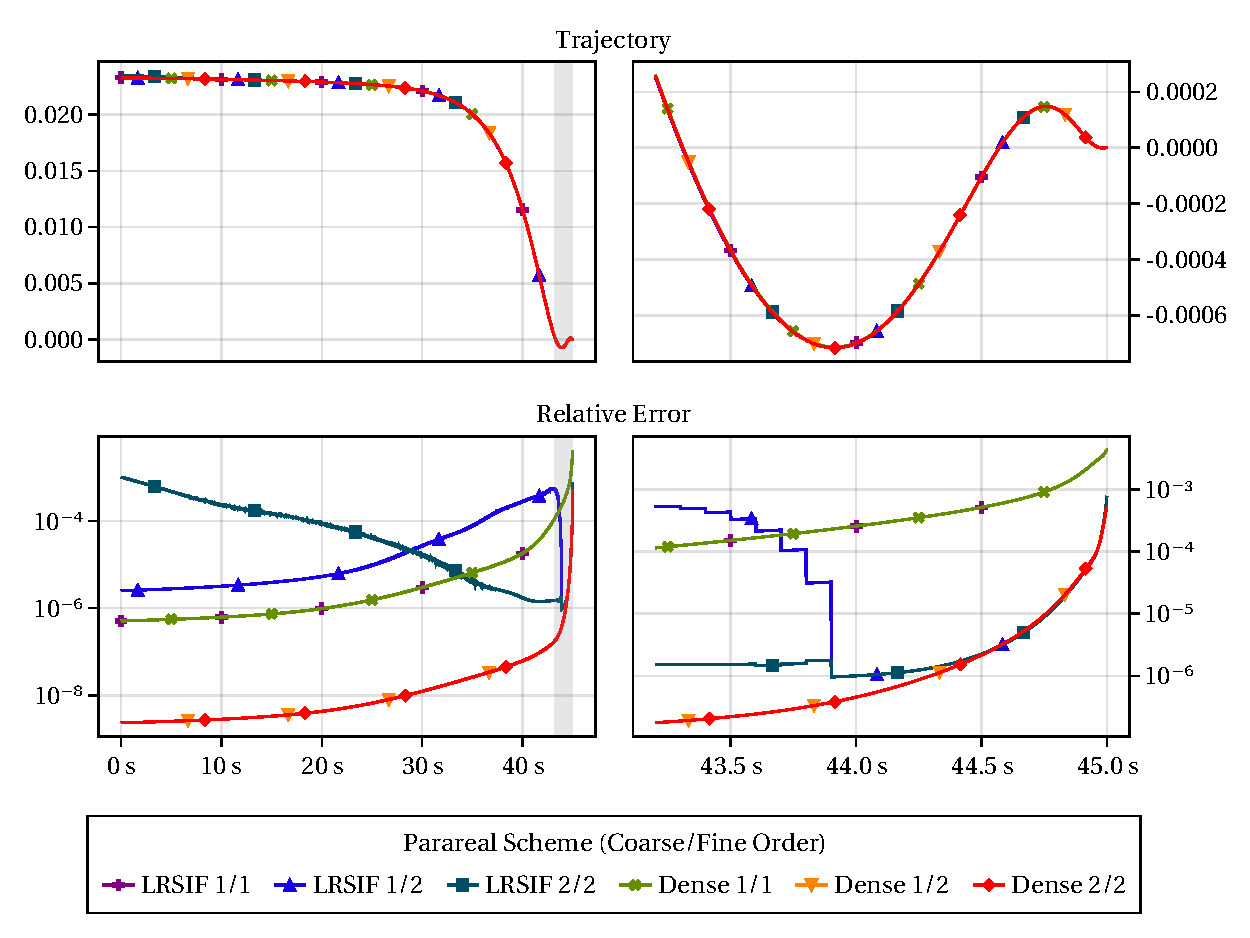
\includegraphics[width=0.9\textwidth]{figures/fig_results_parareal.pdf}%
  \caption{Trajectory $X_{1,77}$ and relative error in $K$ for Rail371}
  \label{fig:7.7}
  \end{figure}
}
\only<+>{
  \begin{figure}
  \renewcommand\thefigure{7.8} % number in thesis
  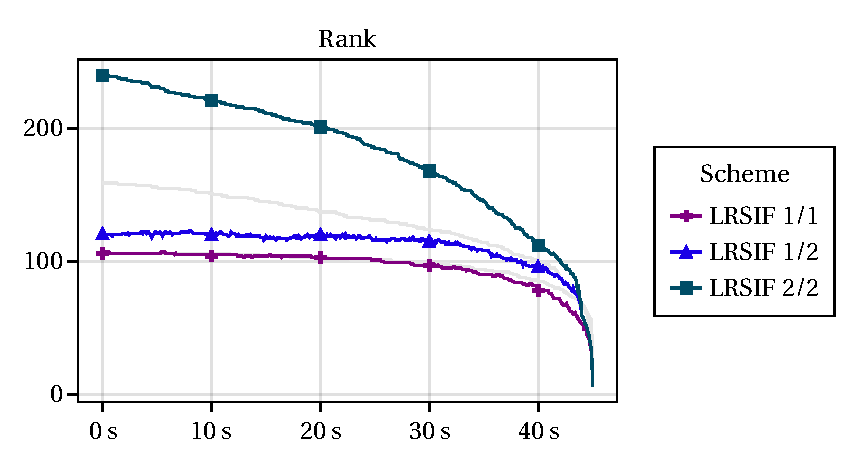
\includegraphics[width=0.9\textwidth]{figures/fig_results_parareal_rank.pdf}%
  \caption{Rank of $X=LDL^\T$ for Rail371}
  \end{figure}
}
\only<+>{
  \begin{figure}
  \renewcommand\thefigure{7.9} % number in thesis
  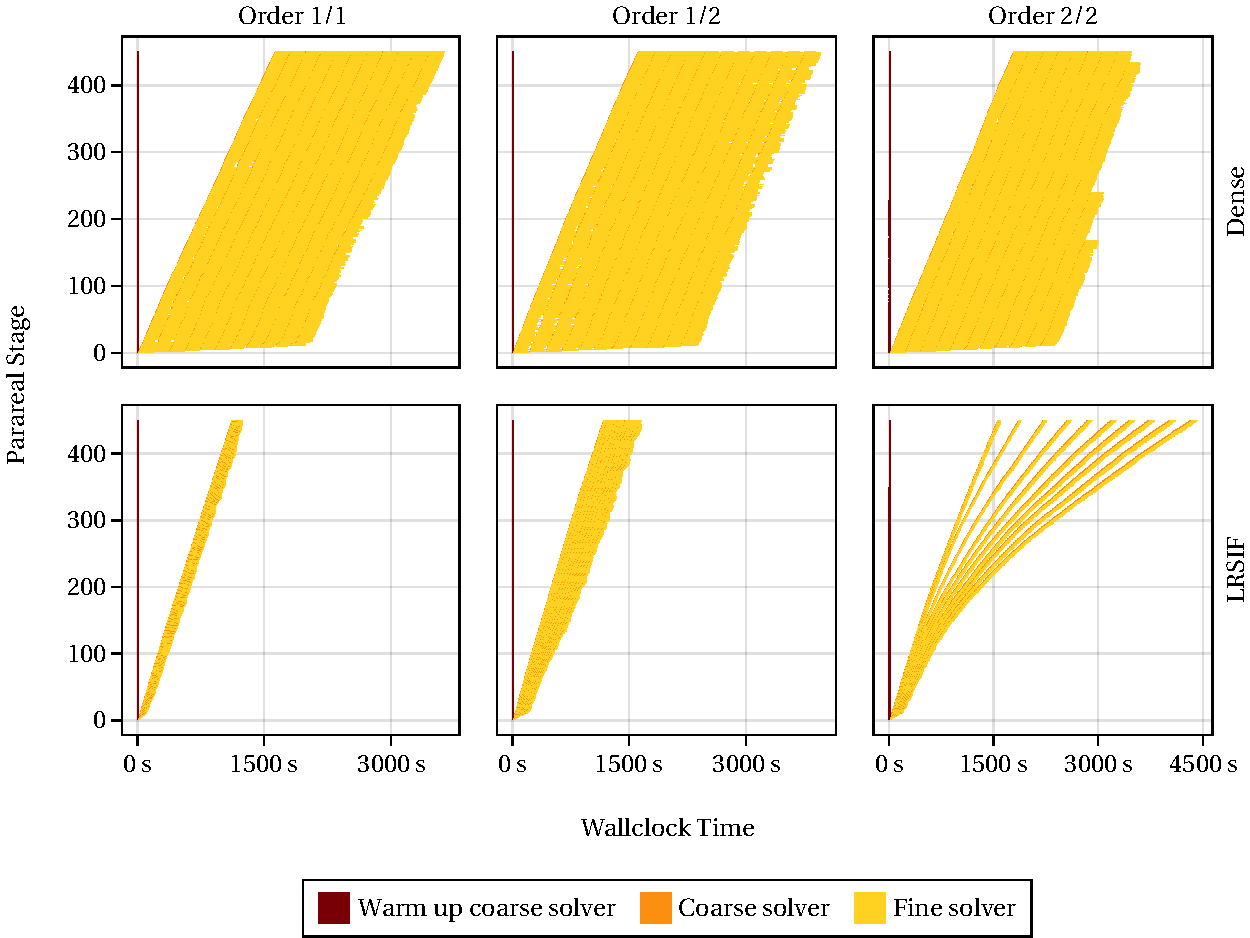
\includegraphics[width=0.85\textwidth]{figures/fig_timeline_all.pdf}%
  \caption{Timeline chart of parareal method applied to Rail371}
  \end{figure}
}
  \end{minipage}
  \column{0.3\textwidth}
  \begin{block}{Parareal Setup}
    \begin{itemize}
      \item
        450 coarse steps (\SI{100}{\milli\second})
      \item
        100 fine steps per coarse step (\SI{1}{\milli\second})
      \item
        Max.~\#iterations: 10
      \item
        Convergence:\\
        relative change in~$X$\\ below $371\umach$,\\
        twice in a row,\\
        max.~1 iteration\\
        behind prev.~stage,\\
        and all previous\\
        stages converged
    \end{itemize}
  \end{block}
  \end{columns}
\end{frame}

\subsection{Parallel Scaling}

\begin{frame}[b,fragile,label=speedup]{\secname}
\framesubtitle{\subsecname}
  \setbeamertemplate{caption}[numbered]
  \begin{columns}[c,onlytextwidth]
  \column{0.65\textwidth}
  \begin{table}
  \setlength{\abovecaptionskip}{0pt}
  %TODO: use hanging captions
  \raggedright
  \renewcommand\thetable{7.3} % number in thesis
  \caption{%
    Speed-up and parallel efficiency of parareal method applied to Rail371 using $N=450$ cores.
    (timings in seconds)
  }
  \begin{tabular}{%
    l
    S[table-format=4.2] % par
    S[table-format=6.2] % seq est
    S[table-format=2.2] % speedup
    S[round-precision=3, round-minimum=0.001, table-format=1.3, table-space-text-post=$^{*}$] % efficiency
  }
    \toprule
    Solver &
    {$\tpar$} &
    {$\hattseq$} &
    {$\frac{\hattseq}{\tpar}$} &
    {$\frac{\hattseq}{N\cdot\tpar}$} \\
    \midrule
    \input{tables/speedup450_lr.tex}
    \addlinespace
    \input{tables/speedup450_de.tex}
    \addlinespace
    \input{tables/speedup450_ref.tex}
    \midrule
    \pause
    Rail1357 & 3001.4058759212494 & 22684.368317604065 & 7.557914275969537 & 0.016795365057710083$^{*}$ \\
    \bottomrule
  \end{tabular}
  \end{table}
  \column{0.35\textwidth}
  \begin{block}{Addendum}
  \begin{itemize}
    \item
      Actual runtime of (sequential) Dense 4:

      $\tseq < \SI{86831}{\second}$

      (Slurm job duration)
    \item
      LRSIF 1/1 applied to Rail1357:
      % TODO: goto button for timeline (and back button there)

      \begin{itemize}
        \item
          2 BLAS threads\\ per process
        \item
          $2\times$ round-robin scheduling onto\\
          $P=225$ processes
        \item[{\makebox[\widthof{\usebeamertemplate{itemize item}}][c]{$\ast$}}]
          actual efficiency:
          $2\hattseq/2P\cdot \tpar = \num[round-precision=3]{0.033590730115420166}$
      \end{itemize}

      % $\tpar = \SI{3600}{\second}$ (Slurm job duration)
  \end{itemize}
  \end{block}
  {\hfill\hyperlink{app:rail1357}{\beamergotobutton{Appendix}}}
  \vspace{-\baselineskip}
  \end{columns}
  \onslide
  \vfill
  \begin{lstlisting}
MY_KIND=dense MY_NF=100 MY_OF=1 MY_OC=1 sbatch -n450 -J de11 par.job
  \end{lstlisting}
\end{frame}

\subsection{Conclusion}

\begin{frame}<1>[label=conclusion]{\secname}
\framesubtitle{\subsecname}
\begin{block}{Parareal Method}
  \begin{itemize}
    \item
      Offers large speed-ups, but has low efficiency
    \item
      Present implementation has severe ramp-up delay

      \uncover<2>{due to Julia's JIT compiler warm-up}
    \item
      Low-rank codes allow/require much smaller (temporal) resolutions

      \uncover<2>{to reach similar speed-ups as dense codes}
    \item
      Runtime of low-rank solvers varies from evaluation to evaluation

      \uncover<2>{due to varying rank and stiffness}
      $\leadsto$ complicates load balancing
  \end{itemize}
\end{block}
\begin{block}{DRE Solvers}
  \begin{itemize}
    \item
      Ros1 performs identically for dense and low-rank data
    \item
      Reproduced issues with low-rank Ros2 in Julia

      \uncover<2>{\cite{Lang2015} had used MATLAB}
  \end{itemize}
\end{block}
\end{frame}

\begin{frame}<1>[label=conclusion]{\secname}
\framesubtitle{Open Problems}
\begin{block}{ParaReal.jl}
  \begin{itemize}
    \item
      Currently limited to processes as executors
    \item
      Lacks asynchronous communication
    \item
      How to eliminate the ramp-up delay?

      \uncover<2>{\ie compile more code ahead-of-time}
    \item
      How to improve load balancing?

      \uncover<2>{%
      \eg via round-robin scheduling or threaded oversubscription;\\
      but how to handle threads \& processes?
      }
  \end{itemize}
\end{block}
\begin{block}{DifferentialRiccatiEquations.jl}
  \begin{itemize}
    \item
      Needs to record more metrics
    \item
      \texttt{\LDLt} (and \texttt{LowRankUpdate}) types could be separated into their own packages
  \end{itemize}
\end{block}
\end{frame}


\section{Summary}

\begin{frame}
  \frametitle{Summary}
  foo
\end{frame}

\appendix

\documentclass[
  aspectratio=1610,
]{beamer}

%\includeonlyframes{current,other}

\usepackage[american]{babel}
\usepackage[utf8]{inputenc}
\usepackage[T1]{fontenc}

% needs https://tex.stackexchange.com/questions/423848/xelatex-xy-and-dejavu-otf#423854
%\usepackage{dejavu-otf} % default Makie font: DejaVu Sans
%\usefonttheme{professionalfonts}

\title{A Low-Rank Parareal Solver for\\ Differential Riccati Equations\\ Written in Julia}
\author{Jonas Schulze}
\institute{Faculty of Mathematics\\ Otto-von-Guericke-Universität Magdeburg}
\date{May 10, 2022}
\subject{subject}

% beamer appearance
\setbeamercolor{block body}{bg=mpi} % for debugging
\setbeamercovered{transparent}
\beamertemplatenavigationsymbolsempty

\newcommand\maketocframe[1][]{%
  \begin{frame}{Outline}
    \tableofcontents[#1]
  \end{frame}
}

\AtBeginSection{%
  \maketocframe[currentsection,currentsubsection]
}

\usepackage[
  style=authoryear,
]{biblatex}
\addbibresource{stuff.bib}

\input{preamble/packages-slides}
\input{preamble/math.tex}
\input{preamble/other.tex}
\input{preamble/abbreviations}
\input{preamble/drawing}

\renewcommand\mathrm\mathsf % fix \umach
\newcommand\emptyblock[1]{%
  \begin{beamercolorbox}{block title}
    \usebeamerfont{block title}%
    #1
  \end{beamercolorbox}
}

%TODO: what if the frame needs multiple slides?
\newcommand\bigpicture[1]{%
  \begin{block}{Big Picture}
    \begin{itemize}
      \item
        Differential \Riccati Equation (DRE)
      \ifnum#1<2 \pause\fi
      \item
        Solution in LRSIF
      \ifnum#1<3 \pause\fi
      \item
        Rosenbrock method\\ to solve DRE
      \ifnum#1<4 \pause\fi
      \item
        Rosenbrock stages are ALEs
      \ifnum#1<5 \pause\fi
      \item
        ADI method\\ to solve ALE
      \ifnum#1<6 \pause\fi
      \item
        Parareal method\\ for speed-up
    \end{itemize}
  \end{block}
}

\newcommand\tallcmat[1]{\tikz[baseline=-0.5ex]\node[tallmat,fill=#1] {};}
\newcommand\smallcmat[1]{\tikz\node[smallmat,fill=#1] {};}
\newcommand\widecmat[1]{\tikz\node[widemat,fill=#1] {};}
\newcommand\colorldlt[1]{%
  \mathop{\tallcmat{#1}}
  \mathop{\smallcmat{#1}}
  \mathop{\widecmat{#1}}
}

\newcommand\colorspacing{%
  \arraycolsep=3pt
  \def\arraystretch{0.75}
}

\begin{document}

\frame[plain]{\titlepage}
\maketocframe

\everymath{\displaystyle}

\input{content/slides_motivation}

\section{Next}

\input{content/slides_lrsif}
\input{content/slides_rosenbrock}
\input{content/slides_parareal}
\input{content/slides_results}

\section{Summary}

\begin{frame}
  \frametitle{Summary}
  foo
\end{frame}

\appendix

\input{appendix/slides}

\end{document}


\end{document}


\end{document}


\end{document}
